\documentclass[preprint,11pt]{elsarticle}
\usepackage{amsmath,amssymb}
\usepackage{amsthm}
\usepackage{url}
\usepackage{graphicx}

\newtheorem{theorem}{Theorem}[section]
\newtheorem{corollary}[theorem]{Corollary}
\newtheorem{lemma}[theorem]{Lemma}
\newtheorem{proposition}[theorem]{Proposition}
\theoremstyle{definition}
\newtheorem{example}[theorem]{Example}
\newtheorem{definition}[theorem]{Definition}
\theoremstyle{remark}
\newtheorem{remark}[theorem]{Remark}

\DeclareMathOperator{\ord}{ord}
\DeclareMathOperator{\Fix}{Fix}
\DeclareMathOperator{\Irr}{Irr}
\DeclareMathOperator{\Aut}{Aut}
\newcommand{\Z}{\mathbb Z}
\newcommand{\Q}{\mathbb Q}
\newcommand{\ii}{\mathrm i}
\makeatletter
\newcommand{\SR}[1]{\@nameuse{SR@#1}}
\makeatother
\expandafter\def\csname SR@app:fam\endcsname{S1}
\expandafter\def\csname SR@app:normal\endcsname{S3}
\expandafter\def\csname SR@lem:kgen\endcsname{S1.3}
\expandafter\def\csname SR@prop:dic\endcsname{S1.1}
\expandafter\def\csname SR@prop:k4fam\endcsname{S1.4}
\expandafter\def\csname SR@rem:dic\endcsname{S1.2}
\expandafter\def\csname SR@rem:kgen\endcsname{S1.6}
\expandafter\def\csname SR@sec:normal\endcsname{S2}
\expandafter\def\csname SR@tab:normal\endcsname{S1}
\expandafter\def\csname SR@thm:C\endcsname{S2.1}
\expandafter\def\csname SR@lem:Cn\endcsname{S3.2}
\expandafter\def\csname SR@prop:mst\endcsname{S3.3}

\journal{Discrete Mathematics}

% >>> EDIT HERE before submission: replace the text below by the DOI/URL of the data archive (Zenodo / Mendeley Data) <<<
\newcommand{\ArchiveLink}{[repository and DOI to be inserted]}

\emergencystretch=2em
\begin{document}


\begin{frontmatter}

\title{Perfect state transfer from Hermitian weighing matrices: mixed Cayley graphs over groups with an abelian subgroup of index $2$}

\author{Afsaneh Khalilipour\corref{mycorrespondingauthor}}
\cortext[mycorrespondingauthor]{Corresponding author}
\ead{khalilipour.afsaneh@gmail.com}

\address{Department of Mathematics, Faculty of Science, Shahid Rajaee Teacher Training University, Tehran, 16785-163, I. R. Iran}

\begin{abstract}
Let $\mathrm{Cay}(G,S)$ be a mixed Cayley graph in which every vertex lies on $\zeta>0$ undirected edges, and let $c\in S\cap S^{-1}$ be a central involution. Write $H$ for the Hermitian adjacency matrix and $L_c$ for the permutation matrix of $v\mapsto cv$. We show that perfect state transfer (PST) from every vertex $g$ to $gc$ at time $\pi/2$ occurs if and only if the spectrum of $K=H-L_c$ lies in a single residue class modulo $4$. In the extreme case $\operatorname{spec}(K)=\{k,-k\}$, that is, $K^2=k^2I$ with $k$ even, $K$ is a Hermitian weighing matrix with entries in $\{0,1,\pm\mathrm i\}$ developed over $G$. This mechanism needs arcs: if $K$ is the adjacency matrix of an undirected graph and $K^2=k^2I$, then $k=1$. For $G=A\rtimes_f\mathbb Z_2$ with $A$ abelian, we ask when such a graph is not a Cayley graph of any abelian group. For normal connection sets this never happens. For non-normal sets we construct an infinite family on the dihedral groups $D_n$ ($n\ge6$ even), the smallest member having $12$ vertices, whose members are graphical regular representations in the mixed sense. Further families on $\mathrm{Dic}_n$, $SD_{2^k}$ and $\mathrm{Dih}(\mathbb Z_4\times\mathbb Z_{4m})$ are proved in a supplementary note. The corresponding question for undirected graphs remains open. On generalised dicyclic groups we give a Fourier criterion for weighing sets of every weight and classify the sets of weight $2$. Weight-$4$ sets exist on $\mathrm{Dic}_n$ for every $n\ge5$ and do not exist for $n=3,4$, whereas a computer search finds none on $D_n$ for $n\le34$. An exhaustive enumeration over the non-abelian groups of order at most $16$ with an abelian subgroup of index $2$ yields no such graph on fewer than $12$ vertices. As background, we prove that in every vertex-transitive mixed graph with $\zeta>0$, PST forces an integral spectrum and a central automorphism of order $2$ or $4$.
\end{abstract}

\begin{keyword}
perfect state transfer \sep mixed Cayley graph \sep Hermitian adjacency matrix \sep weighing matrix \sep abelian subgroup \sep graphical regular representation

\MSC[2020] 05C25 \sep 05C50 \sep 81P45
\end{keyword}

\end{frontmatter}


\section{Introduction}

The continuous-time quantum walk on a graph with Hermitian adjacency matrix $H$ evolves by $U(t)=\exp\bigl(-\ii tH\bigr)$. The graph has \emph{perfect state transfer} (PST) from $u$ to $v\ne u$ at time $\tau>0$ if $|U(\tau)_{vu}|=1$ \cite{Bose,Christandl}, and \emph{multiple state transfer} (MST) on a vertex set $X$ if PST occurs between any two distinct vertices of $X$ \cite{GodsilLato,SongLin}. We work with \emph{mixed} graphs, which have both undirected edges and directed arcs: $H_{uv}=1$ for an edge $uv$, $H_{uv}=\ii=-H_{vu}$ for an arc $u\to v$, and $H_{uv}=0$ otherwise \cite{Liu,Guo}. Arcs change the arithmetic of transfer: the transfer permutation can have order $4$, and PST from $u$ to $v$ need not be followed by PST from $v$ to $u$ at the same time \cite{SongLinEJC}.

PST is a property of a graph, not of a presentation of it as a Cayley graph \cite{AG}. Let $G=A\rtimes_f\Z_2$ with $A$ abelian of index $2$. An undirected $\mathrm{Cay}(G,S)$ is also a Cayley graph of an abelian group whenever some element of $G\setminus A$ normalises $S$. This covers conjugation-closed sets, PST whose involution is a translation by an element outside $A$, and generalised dihedral groups with both parts of $S$ inverse-closed \cite{AG,MS}. According to \cite{AG}, the explicit constructions of PST on dihedral, dicyclic, generalised dihedral and $V_{8n}$ groups that it examines are therefore abelian Cayley graphs in non-abelian presentations, and so is every connected vertex-transitive graph with PST on at most $22$ vertices \cite[Section~6]{AG}. Genuinely non-abelian examples on groups with an abelian subgroup of index $2$ are found in \cite{AG} by computer search (a Cayley graph of $D_{48}$, and graphical regular representations on $32$ vertices). No infinite family is given, and \cite[Problem~8.2]{AG} asks whether infinitely many such representations exist.

Mixed graphs are not an arbitrary detour. If $H$ is real, then $U(t)=\exp\bigl(-\ii tH\bigr)$ is symmetric, so $|U(t)_{uv}|=|U(t)_{vu}|$ for all $u,v$ and $t$. Arcs make $H$ non-real and remove this constraint: Hermitian adjacency matrices of mixed graphs are Hamiltonians of chiral quantum walks with phases $0$ and $\pm\pi/2$ on the edges, a model that breaks time-reversal symmetry \cite{Lu,Acuaviva}. Here the arcs also play a structural role, because the mechanism of Section~\ref{sec:nn} cannot work without them (Remark~\ref{rem:mixedonly}).

We therefore ask the corresponding question for mixed graphs. Throughout, $G=A\rtimes_f\Z_2$ with $f\ne\mathrm{id}$, and $S$ is an arbitrary connection set with $\zeta=|S\cap S^{-1}|>0$, so that every vertex lies on an undirected edge. Which mixed Cayley graphs on $G$ have PST, and when is the graph not a Cayley graph of any abelian group? The hypothesis $\zeta>0$ is what forces an integral spectrum; for $\zeta=0$ the transfer permutation can have order $3$, and order $6$ is not excluded by the general theory \cite{CPRS}.

\medskip\noindent\emph{Scope.} These questions concern mixed graphs. Problem~8.2 of \cite{AG} concerns undirected graphs, and we do not answer it: the weighing mechanism cannot produce undirected examples (Remark~\ref{rem:mixedonly}), and the graphs $\Gamma_n$ of Proposition~\ref{prop:Dn} are regular only in the mixed sense (Remark~\ref{rem:grr-checks}(iii)). The hypothesis $c\in S$ does not separate the two settings: by Remark~\ref{rem:toggle} the criterion of Theorem~\ref{thm:pi2} also holds for $c\notin S$, and the undirected representation on $32$ vertices displayed in \cite[Section~6.1]{AG} is of that kind.

\medskip\noindent\emph{What is known and what is new.} Theorem~\ref{thm:G} is the Hermitian analogue of Godsil's theorem for undirected vertex-transitive graphs \cite{GodsilPeriodic,GodsilSTG}. The theory of normal connection sets (Section~\SR{sec:normal}) parallels \cite{CPRS}. The reduction to abelian groups (Theorem~\ref{thm:B}) extends \cite[Lemmas~5.1 and~5.2]{AG} from undirected to mixed graphs, and the block decomposition (Theorem~\ref{thm:N}) extends the block method of \cite{Arezoomand,BehajainaLegrand}. These results are included with complete proofs because later sections use them. The $\pi/2$ criterion and the weighing condition (Theorems~\ref{thm:pi2} and~\ref{thm:weighing}) follow directly from the identity $\exp\bigl(-\ii(\pi/2)L_c\bigr)=-\ii L_c$, the left-translation symmetry of $H$ and the spectral theorem; their role is to reduce transfer at time $\pi/2$ to a condition on $K=H-L_c$ alone. The contributions of this paper are what is proved under that condition: the infinite family of Proposition~\ref{prop:Dn} and the results of Propositions~\SR{prop:dic} and~\SR{prop:k4fam} in Section~\SR{app:fam}; the Fourier criterion, the classification of weight $2$ and the weight-$4$ family on $\mathrm{Dic}(A,y)$ (Theorems~\ref{gd:fourier} and~\ref{gd:k2}, Proposition~\ref{gd:k4}); and the exhaustive data on the non-abelian groups of order at most $16$ with an abelian subgroup of index $2$ (Appendix~\ref{sec:search}). Results whose number carries the prefix S are proved in the supplementary note \cite{Supp}; all other results are proved in this paper. The unrefereed arXiv preprints \cite{AG,DihNew,CPRS} are cited only for context, for comparison of results and for the open problems we address. No statement proved here uses a result from them as an input: the oriented set of \cite[Theorem~8.2]{CPRS} used in Proposition~\SR{prop:mst} is treated again from scratch in Lemma~\SR{lem:Cn}.

\medskip\noindent\emph{A spectral criterion and weighing matrices.} If $c\in S\cap S^{-1}$ is a central involution, then PST from every $g$ to $gc$ at time $\pi/2$ occurs if and only if all eigenvalues of $H-L_c$ lie in one residue class modulo $4$ (Theorem~\ref{thm:pi2}). The extreme case is $\operatorname{spec}(K)=\{k,-k\}$ for $K=H-L_c$, that is, $K^2=k^2I$ with $k$ even. Then $K$ is a Hermitian weighing matrix with entries in $\{0,1,\pm\ii\}$ developed over $G$, and $U(\pi/2)=(-1)^{k/2+1}\ii R_c$ (Theorem~\ref{thm:weighing}). (Two eigenvalues alone do not force $K^2=k^2I$: for $G=\Z_2^3$ and $S'=\{(1,0,0),(0,1,0),(1,1,0)\}$, $c=(0,0,1)$, one has $K=K_4\sqcup K_4$ with spectrum $\{3,-1\}$, all in one class modulo $4$.) This mechanism is intrinsically mixed: an undirected $K$ with $K^2=k^2I$ has $k=1$ (Remark~\ref{rem:mixedonly}).

\emph{Non-abelian examples.} A commutation test (Lemma~\ref{lem:abtest}) certifies that a graph is not a Cayley graph of any abelian group. It applies to an infinite family on $D_n$ ($n\ge6$ even), the smallest member having $12$ vertices, and, in Section~\SR{app:fam}, to families on $\mathrm{Dic}_n$ ($n\ge3$), $SD_{2^k}$ ($k\ge4$) and $\mathrm{Dih}(\Z_4\times\Z_{4m})$ ($m\ge3$). On $D_n$ the automorphism group of the graph is $L(D_n)$, so these are graphical regular representations in the mixed sense (Proposition~\ref{prop:Dn}). Normal connection sets never give such examples, since the graph is then a Cayley graph of an abelian group (Theorem~\ref{thm:B}).

\emph{Dihedral versus dicyclic.} On $\mathrm{Dic}(A,y)$, two Fourier conditions characterise weighing sets of every weight (Theorem~\ref{gd:fourier}), and the weight-$2$ sets are listed (Theorem~\ref{gd:k2}). Weight $4$ separates the two families: weight-$4$ sets exist on $\mathrm{Dic}_n$ for every $n\ge5$ and do not exist for $n=3,4$, whereas a search finds none on $D_n$ for $n\le34$ (Corollary~\ref{gd:dicn}, Remark~\SR{rem:kgen}).

\emph{Background results.} In every vertex-transitive mixed graph with $\zeta>0$, PST forces an integral spectrum and a central automorphism of order $2$ or $4$, and periodicity is equivalent to integrality (Theorem~\ref{thm:G}). On $A\rtimes_f\Z_2$, PST is governed by $2\times2$ Hermitian blocks indexed by the characters of $A$ (Theorem~\ref{thm:N}); for undirected $S$ this is the block criterion of Arezoomand \cite{Arezoomand}. For normal sets the theory reduces to characters, and for every $n\ge5$ the modular group $M_{2^n}$ carries a connected normal mixed set with $\zeta=8$ and multiple state transfer on four vertices (Section~\SR{app:normal}).

\emph{Related work.} PST on Cayley graphs has been described for abelian groups \cite{Basic,ArnadottirGodsil,TFC}, for normal sets on dihedral and dicyclic groups \cite{CF,DihNew,ASG}, for Cayley graphs over semi-dihedral groups \cite{LCWW}, and, for undirected sets on groups with an abelian subgroup of index $2$, through semi-Cayley graphs \cite{Arezoomand} (see also \cite{WangFeng}). For mixed graphs, integral mixed Cayley graphs on such groups are studied in \cite{BehajainaLegrand}, PST and MST on abelian groups in \cite{KG}, oriented normal Cayley graphs on arbitrary groups in \cite{CPRS}, and circulants and the general theory in \cite{SongOriented,SongLin,SongLinEJC,GodsilLato,Cameron,Acuaviva}; see also \cite{SongClasses} for the transfer times of complete PST classes in mixed graphs.

\emph{Group-developed weighing matrices.} A $G$-developed weighing matrix of weight $k$ is an element $X\in\Z[G]$ with coefficients in $\{0,\pm1\}$ and $XX^{(-1)}=k$. Over abelian $G$ these have been studied extensively, in particular for cyclic $G$ \cite{AH}; the equation makes sense for every finite group \cite{LS}. Group developments over arbitrary finite groups occur as a special case of the cohomology-developed weighing matrices of \cite{GD}. Complex generalised weighing matrices (entries in $\{0\}\cup\mu_m$) that are invariant under a regular group action are studied in \cite{CdL}; see \cite{Egan} for a survey. The matrix $K=H-L_c$ is of this type with $m=4$: it is a Hermitian weighing matrix with entries in $\{0,1,\pm\ii\}$ developed over $G=A\rtimes_f\Z_2$. What distinguishes our setting is the question asked of it. We ask when $K$ is not developed over any abelian group, which is equivalent to the mixed Cayley graph not being a Cayley graph of an abelian group, and we link the weighing condition to perfect state transfer through Theorems~\ref{thm:pi2} and~\ref{thm:weighing}. Complex weighing matrices of a given weight fall within that framework; the new results here are the families of Proposition~\ref{prop:Dn} and of Section~\SR{app:fam}, the Fourier criterion and classification on $\mathrm{Dic}(A,y)$, and the exhaustive data of Appendix~\ref{sec:search}.

\emph{Organisation.} Sections~\ref{sec:groups}--\ref{sec:block} set up the tools: the structure theorem, the reduction to abelian groups with its commutation test, and the block decomposition. Section~\ref{sec:nn} contains the $\pi/2$ criterion and the dihedral family $\Gamma_n$, and Section~\ref{sec:gd} the Fourier criterion with the classification of weights $2$ and $4$. Appendix~\ref{app:G} proves the structure theorem, and Appendices~\ref{sec:search} and~\ref{sec:comp} give the exhaustive data and the method. Material that no proof in the main text uses is in a separate supplementary note \cite{Supp}: the theory of normal connection sets, the families on $\mathrm{Dic}_n$, $SD_{2^k}$ and $\mathrm{Dih}(\Z_4\times\Z_{4m})$, and the data for weight $k>2$. Numbers prefixed by S refer to that note.

\section{Groups with an abelian subgroup of index $2$}\label{sec:groups}

Let $A$ be a finite abelian group (additive), $f\in\mathrm{Aut}(A)$ with $f^2=\mathrm{id}$, and $y\in A$ with $f(y)=y$. Let $G=A\rtimes_f\Z_2$ be $A\times\{0,1\}$, with $(a,r)$ standing for $x^ra$, where $x^2=y$ and $x^{-1}ax=f(a)$:
\begin{align*}
(a,0)(b,0)&=(a+b,0), & (a,0)(b,1)&=(f(a)+b,1),\\
(a,1)(b,0)&=(a+b,1), & (a,1)(b,1)&=(y+f(a)+b,0).
\end{align*}
(The last rule follows from $xaxb=x^2(x^{-1}ax)b$.) Inverses: $(a,0)^{-1}=(-a,0)$ and $(a,1)^{-1}=(-f(a)-y,\,1)$. For $y\ne0$ the term $-y$ is essential; it matters for $U_{6n}$ and for the dicyclic and quaternion-type groups. Conversely, if $A\le G$ is abelian of index $2$ and $x\in G\setminus A$, then $f(a)=x^{-1}ax$ and $y=x^2$ have the above properties, so every group with an abelian subgroup of index $2$ is of this form. Table~\ref{tab:groups} lists the standard groups used below. $G$ is non-abelian if and only if $f\ne\mathrm{id}$, and this is assumed throughout.

\begin{table}[ht]
\centering
\small
\begin{tabular}{lccc}
Group & $A$ & $f$ & $y$\\\hline
dihedral $D_n$ (order $2n$) & $\Z_n$ & $-\mathrm{id}$ & $0$\\
dicyclic $\mathrm{Dic}_n$ (order $4n$) & $\Z_{2n}$ & $-\mathrm{id}$ & $n$\\
semidihedral $SD_{2^k}$ & $\Z_{2^{k-1}}$ & $(2^{k-2}-1)\cdot$ & $0$\\
modular $M_{2^k}$ & $\Z_{2^{k-1}}$ & $(2^{k-2}+1)\cdot$ & $0$\\
$U_{6n}=\langle a,b\mid a^{2n}=b^3=1,a^{-1}ba=b^{-1}\rangle$ & $\Z_n\times\Z_3$ & $(\mathrm{id},-\mathrm{id})$ & $(1,0)$ ($x=a$)\\
$(\Z_4\times\Z_4)\rtimes\Z_2$ & $\Z_4^2$ & swap & $0$
\end{tabular}
\caption{Standard groups $G=A\rtimes_f\Z_2$ in the notation of this section: the group, the abelian subgroup $A$ of index $2$, the automorphism $f$ and the element $y=x^2$.}\label{tab:groups}
\end{table}

\begin{lemma}\label{lem:center}
If $f\ne\mathrm{id}$ then $Z(G)=\Fix(f):=\{a\in A:f(a)=a\}$; in particular $y\in Z(G)$ and no element outside $A$ is central.
\end{lemma}
\begin{proof}
$(b,0)(a,1)=(f(b)+a,1)$ and $(a,1)(b,0)=(a+b,1)$, so an element $(a,1)$ commutes with all of $A$ only if $f=\mathrm{id}$. For $a\in A$: $(a,0)(0,1)=(f(a),1)$ and $(0,1)(a,0)=(a,1)$, so $a$ is central iff $f(a)=a$. Finally $f(y)=y$.
\end{proof}
\section{Mixed Cayley graphs and a structure theorem for arbitrary connection sets}\label{sec:G}

Let $G$ be a finite group and $S\subseteq G\setminus\{1\}$ a connection set. Put $S_u=S\cap S^{-1}$, $T=S\setminus S^{-1}$, $\zeta=|S_u|$ and $N_G(S)=\{g\in G:\ g^{-1}Sg=S\}$. The graph $\Gamma=\mathrm{Cay}(G,S)$ has vertex set $G$, an undirected edge $\{g,h\}$ when $g^{-1}h\in S_u$, and an arc $g\to h$ when $g^{-1}h\in T$; so $H_{g,h}=1,\ii,-\ii,0$ according as $g^{-1}h\in S_u$, $T$, $T^{-1}$, or else. Write $L_g:e_v\mapsto e_{gv}$ and $R_g:e_v\mapsto e_{vg}$ for the permutation matrices on the basis $(e_v)_{v\in G}$ of $\mathbb C^G$. Throughout, we assume that $\zeta>0$.
\begin{lemma}\label{lem:symL}
$L_g$ commutes with $H$, hence with $U(t)$; so $\Gamma$ is vertex-transitive. Consequently, for every polynomial $p$, $p(H)=0$ iff $p(H)e_1=0$.
\end{lemma}
\begin{proof}
$(gu)^{-1}(gv)=u^{-1}v$. If $p(H)e_1=0$ then $p(H)e_g=p(H)L_ge_1=L_gp(H)e_1=0$ for all $g$.
\end{proof}

\begin{theorem}[Structure theorem]\label{thm:G}
Let $\Gamma$ be a mixed graph with Hermitian adjacency matrix $H$ whose group $\mathrm{Aut}(\Gamma)$ of automorphisms (preserving edges and the directions of arcs) is transitive on the vertices, and let $\zeta>0$ be the number of undirected edges at a vertex. For a spectrum that is integral put $\gamma=\gcd\{\theta-\zeta:\ \theta\text{ an eigenvalue of }H,\ \theta\ne\zeta\}$, a positive integer.
\begin{enumerate}
\item[(P)] \emph{Periodicity.} Call $\Gamma$ periodic at a vertex $u$ if $|U(t)_{uu}|=1$ for some $t>0$. The following are equivalent: (i) $\Gamma$ is periodic at some vertex; (ii) $U(t)$ is a scalar matrix for some $t>0$; (iii) the spectrum of $H$ is integral. In this case $U(t)$ is scalar exactly for $t\in(2\pi/\gamma)\Z$, and $U(2\pi k/\gamma)=\exp\bigl(-2\pi\ii k\zeta/\gamma\bigr)I$.
\end{enumerate}
Suppose moreover that PST from $u$ to $v\ne u$ occurs at time $\tau$. Then:
\begin{enumerate}
\item[(a)] $U(\tau)=\exp\bigl(-\ii\tau\zeta\bigr)P_\sigma$, where $P_\sigma$ is the permutation matrix of a fixed-point-free permutation $\sigma\in Z(\mathrm{Aut}(\Gamma))$ with $\sigma(u)=v$. Thus PST occurs between $w$ and $\sigma(w)$ for every vertex $w$. If $\Gamma=\mathrm{Cay}(G,S)$ (no normality is assumed), $u=1$ and $v=z$, then $\sigma(g)=gz$, that is, $U(\tau)e_g=\exp\bigl(-\ii\tau\zeta\bigr)e_{gz}$ for all $g\in G$, and $z\in Z(N_G(S))$.
\item[(b)] The spectrum of $H$ is integral and $\tau\in2\pi\Q$.
\item[(c)] $\sigma^4=1$, so $\ord(\sigma)\in\{2,4\}$, and $\ord(\sigma)=2$ if $\Gamma$ is undirected. In particular the number of vertices is even.
\item[(d)] Let $\Lambda=\{t\in\mathbb R:\ U(t)e_u\in\mathbb Ce_w\text{ for some vertex }w\}$. Then $\Lambda=\tau_0\Z$, where $\tau_0$ is the least time of PST from $u$, and $t\mapsto\sigma_t$ (defined by $U(t)=\lambda_tP_{\sigma_t}$) is a homomorphism of $\Lambda$ onto the cyclic subgroup $\langle\sigma_{\tau_0}\rangle$ of $Z(\mathrm{Aut}(\Gamma))$, which has order $2$ or $4$. The least $t>0$ with $U(t)e_u\in\mathbb Ce_u$ is $|\langle\sigma_{\tau_0}\rangle|\,\tau_0=2\pi/\gamma$. For $\Gamma=\mathrm{Cay}(G,S)$ and $u=1$, the set $S_1^{\rm st}=\{w:\ U(t)e_1\in\mathbb Ce_w\text{ for some }t>0\}$ equals $\langle z_0\rangle$, where $z_0$ is the target at time $\tau_0$; it is a cyclic subgroup of $Z(N_G(S))$ of order $2$ or $4$, $S_g^{\rm st}=gS_1^{\rm st}$ for all $g$, and $U(\tau_0)=\exp\bigl(-\ii\tau_0\zeta\bigr)R_{z_0}$.
\item[(e)] Every time of PST from $u$ has the form $\tau=\pi\ell/(2\gamma)$ with $\ell\in\Z_{>0}$ and $4\nmid\ell$, and the least such time has $\ell\in\{1,2\}$, where $\ell=1$ if and only if $\ord(\sigma)=4$.
\end{enumerate}
\end{theorem}

\begin{remark}[Relation to earlier work]\label{rem:lit}
Theorem~\ref{thm:G} is the Hermitian analogue of Godsil's theorem for undirected vertex-transitive graphs \cite{GodsilPeriodic,GodsilSTG}. The passage from permutation matrices to roots of unity is the argument of \cite[Cor.~2.3]{CPRS}: if $PE=\omega E$ for a permutation matrix $P$ and a spectral idempotent $E$, then $\omega$ lies in the field generated by the entries of $E$. Here that field is $\Q(\ii)$, which allows order $4$. Part~(P) shows that periodicity needs no choice of target: a mixed Cayley graph with $\zeta>0$ is periodic if and only if it is integral, for every finite group. Integrality of the spectrum under PST is derived, not assumed: it follows from $U(\tau)=\lambda R_z$ and $\mathrm{tr}\,H=0$, and this is the only place where $\zeta>0$ enters. For abelian groups, the order restriction and the equivalence of periodicity and integrality are proved in \cite{KG}. If $\ord(\sigma)=4$, transfer from $u$ to $\sigma(u)$ at time $\tau$ returns only at $3\tau$, since $U(3\tau)=\lambda^3P_{\sigma^{-1}}$. For $\mathrm{Cay}(G,S)$ without normality, the transfer is a translation by an element of $Z(N_G(S))$, which need not be central in $G$; the distinction between left and right translations is the point of \cite[Section~3]{AG}.
\end{remark}

\begin{remark}[Integrality is necessary, not sufficient]\label{rem:int}
For normal sets the exact condition is Theorem~\SR{thm:C}. In $M_{16}$ all $485$ normal sets with $\zeta>0$ are integral, yet only $254$ have PST; in $U_{24}$, $485$ of $1967$ are integral and $26$ have PST; in each of $U_{18}$ and $U_{30}$ there are $31$ integral sets and none has PST (Table~\SR{tab:normal}).
\end{remark}

\section{Reduction to abelian groups}\label{sec:red}

Left translations always preserve edges and arcs, and the right translation by $g$ does so if and only if $g$ normalises $S$ (Section~\ref{sec:G}). This gives the following reduction of mixed Cayley graphs on $A\rtimes_f\Z_2$ to abelian groups; it applies in particular to all normal connection sets.

\begin{theorem}[Reduction to abelian groups]\label{thm:B}
Let $G=A\rtimes_f\Z_2$, let $S\subseteq G\setminus\{1\}$ be arbitrary and $\Gamma=\mathrm{Cay}(G,S)$.
\begin{enumerate}
\item[(a)] If there is $g\in N_G(S)\setminus A$, then $g^2\in\Fix(f)\subseteq Z(G)$ and $P=\langle L_a\ (a\in A),\,R_g\rangle$ is an abelian regular subgroup of $\mathrm{Aut}(\Gamma)$, isomorphic to $\bar A_{g^2}=(A\oplus\Z)/\langle(-g^2,2)\rangle=\langle A,\xi\mid\xi^2=g^2\rangle$, which is abelian of order $|G|$. The map $p\mapsto p(1)$ is an isomorphism of mixed graphs from $\mathrm{Cay}(P,\bar S)$, $\bar S=\{p\in P:\ p(1)\in S\}$, onto $\Gamma$, and it is the identity on $A$. In particular $\Gamma$ is a mixed Cayley graph of an abelian group of order $|G|$, which is $A\times\Z_2$ if $g^2=1$.
\item[(b)] If $S$ is normal, (a) applies with $g=x$, where $G=A\cup xA$, and $\bar A_{x^2}=\bar A_y$ with $y=x^2$. PST and MST from $1$ to $z\in A$ occur in $\Gamma$ if and only if they occur in $\mathrm{Cay}(\bar A_y,\bar S)$.
\item[(c)] If PST occurs from $1$ to a vertex $z\notin A$, then $z\in N_G(S)\setminus A$, so (a) applies. Hence a mixed Cayley graph on $G$ that is not a mixed Cayley graph of any abelian group satisfies $N_G(S)\subseteq A$, and has no PST to vertices outside $A$.
\end{enumerate}
\end{theorem}
\begin{proof}
Let $g\in N_G(S)\setminus A$ and write $g=(a_0,1)$. Then $g^2=(y+f(a_0)+a_0,0)$ and $f(g^2)=y+a_0+f(a_0)=g^2$, so $g^2\in\Fix(f)$, which is central by Lemma~\ref{lem:center} (if $f=\mathrm{id}$, then $G$ is abelian and there is nothing to prove). Since $g^{-1}S^{-1}g=(g^{-1}Sg)^{-1}=S^{-1}$, conjugation by $g$ preserves each of $S_u$, $T$ and $T^{-1}$, so $R_g\in\mathrm{Aut}(\Gamma)$ exactly as in the proof of Theorem~\ref{thm:G}(a); likewise $L_a\in\mathrm{Aut}(\Gamma)$ for every $a\in A$. The permutations $L_a$ commute with one another because $A$ is abelian, and each $L_a$ commutes with $R_g$ by associativity, so $P$ is abelian. Because $g^2$ is central, $R_g^2=R_{g^2}=L_{g^2}$, and therefore $P=\{L_a\}\cup\{L_aR_g\}$ and $|P|\le2|A|=|G|$. The group $\{L_a\}$ maps $1$ onto $A$, while $L_aR_g(1)=ag$ runs over $G\setminus A$; thus $P$ is transitive, and since a transitive abelian permutation group is regular, $|P|=|G|$. The map $A\oplus\Z\to P$, $(a,k)\mapsto L_aR_g^k$, is a surjective homomorphism that kills $(-g^2,2)$, and the corresponding quotient has order $2|A|=|P|$, so $P\cong\bar A_{g^2}$. If $g^2=1$, then $R_g^2=1$ and $R_g\notin\{L_a\}$, because $R_g$ does not preserve $A$; hence $P\cong A\times\Z_2$ in this case.

To see that $\Gamma$ is a Cayley graph of $P$, let $p,q\in P$. Since $p$ is an automorphism, there is an arc $p(1)\to q(1)$ if and only if there is an arc $1\to(p^{-1}q)(1)$, that is, if and only if $(p^{-1}q)(1)\in S$, which means $p^{-1}q\in\bar S$; the same reasoning applies to edges. Hence $p\mapsto p(1)$ is an isomorphism $\mathrm{Cay}(P,\bar S)\to\Gamma$, and it is the identity on $A$ because $L_a(1)=a$. This proves the first assertion of the theorem.

Suppose now that $S$ is normal. Then $N_G(S)=G$ contains $x$, so the above applies with $g=x$, and $\bar A_{x^2}=\bar A_y$. The isomorphism constructed above is the identity on $A\ni z$; it therefore fixes the vertices $1$ and $z$, and it carries the entry $U(t)_{z,1}$ of $\Gamma$ to the corresponding entry of $\mathrm{Cay}(\bar A_y,\bar S)$, which gives the equivalence of PST and of MST in the two graphs. Finally, if PST occurs from $1$ to a vertex $z\notin A$, then $z\in N_G(S)$ by Theorem~\ref{thm:G}(a), so $z\in N_G(S)\setminus A$ and the first assertion applies. Consequently a mixed Cayley graph on $G$ that is not a mixed Cayley graph of any abelian group has $N_G(S)\subseteq A$ and no PST to vertices outside $A$.\qedhere
\end{proof}

\begin{remark}\label{rem:BAG}
For undirected graphs, parts (a) and (b) are \cite[Lemmas~5.1 and~5.2]{AG}, and the generalised dihedral case also follows from \cite{MS}. The arguments carry over to mixed graphs because left translations always preserve edges and arcs, while the right translation by $g$ does so exactly when $g$ normalises $S$. (The paper \cite{AG} defines $\mathrm{Cay}(G,S)$ by $hg^{-1}\in S$, which exchanges the two roles; with our convention $g^{-1}h\in S$, the group $N_G(S)$ plays the part that left translations play there.) Hence a mixed Cayley graph on $G$ that is not an abelian Cayley graph has $N_G(S)\subseteq A$, which is the situation of Proposition~\ref{prop:Dn}. For undirected graphs, \cite[Thm.~5.6]{AG} shows that a non-abelian $G$ of this type has a connected Cayley graph with PST if and only if $4\mid|G|$, in line with Table~\SR{tab:normal}, where $U_{18}$ and $U_{30}$ have no normal PST sets. For mixed sets with $\zeta>0$ on $\Z_n$, $n=6,10,14$, a computer check (script \texttt{check\_zn\_mixed.py} of the archive, which tests all $23$, $431$, $7463$ such sets) shows that the perfect matching $S=\{n/2\}$ is the only PST graph; a proof for mixed graphs is open.
\end{remark}

\begin{lemma}\label{lem:abtest}
Let $G$ be a finite group and $S=S_u\sqcup T$ with $S_u=S\cap S^{-1}$ and $T=S\setminus S^{-1}$. For $s\in G$ let $\rho(s)$ be the $G\times G$ permutation matrix with $\rho(s)_{g,gs}=1$, so that $\rho(s)\rho(s')=\rho(ss')$. If $\mathrm{Cay}(G,S)$ is isomorphic, as a mixed graph, to a Cayley graph of an abelian group, then
\[
\sum_{s\in S_u,\;t\in T}\bigl(\rho(ts)-\rho(st)\bigr)=0,
\]
that is, the multisets $\{ts\}$ and $\{st\}$ $(s\in S_u,\ t\in T)$ of elements of $G$ coincide.
\end{lemma}
\begin{proof}
Let $M_u=\sum_{s\in S_u}\rho(s)$ and $M_a=\sum_{t\in T}\rho(t)$; they are the adjacency matrices of the undirected edges and of the arcs of $\mathrm{Cay}(G,S)$. An isomorphism of mixed graphs preserves these two relations. In $\mathrm{Cay}(B,S')$ with $B$ abelian the corresponding matrices are sums of matrices $\rho'(b)$, which commute pairwise because $\rho'(b)\rho'(b')=\rho'(b+b')$. So $M_uM_a=M_aM_u$. Now $M_aM_u-M_uM_a=\sum_{s,t}(\rho(ts)-\rho(st))$, and the matrices $\rho(g)$, $g\in G$, are linearly independent.
\end{proof}
\begin{remark}
The criterion of Lemma~\ref{lem:abtest} is a sufficient condition for a graph \emph{not} to be a Cayley graph of an abelian group; it is not claimed to be necessary. It is the certificate used for the families on $\mathrm{Dic}_n$, $SD_{2^k}$ and $\mathrm{Dih}(\Z_4\times\Z_{4m})$ and, together with the equality $\mathrm{Aut}(\Gamma_n)=L(G)$ of Proposition~\ref{prop:Dn}(iii), for $\Gamma_n$; for $\Gamma_n$ the equality of the automorphism group alone already decides the question. The graphs counted in Table~\ref{tab:ab} are not certified by this test: each of them is compared by isomorphism with all mixed Cayley graphs of all abelian groups of the same order, which decides the question for those orders.
\end{remark}

The condition of Lemma~\ref{lem:abtest} is necessary, not sufficient.

\begin{remark}\label{rem:Abar}
(i) The abelian groups $\bar A_y$ for the standard groups: $D_n\mapsto\Z_n\times\Z_2$; $M_{2^k},SD_{2^k}\mapsto\Z_{2^{k-1}}\times\Z_2$; $\Z_4^2\rtimes\Z_2\mapsto\Z_4^2\times\Z_2$; $U_{6n}\mapsto\Z_{2n}\times\Z_3$; $\mathrm{Dic}_n\mapsto\Z_{2n}\times\Z_2$ ($n$ even) and $\Z_n\times\Z_4$ ($n$ odd). For $n$ even, replace $\xi$ by $\xi-(n/2)a$, which has order $2$; for $n$ odd, the Sylow $2$-subgroup of $\bar A_y$ has order $4$ and contains $\xi$ of order $4$.

(ii) By Theorem~\ref{thm:B}, for normal sets all spectral and transfer properties are those of mixed Cayley graphs on $\bar A_y$. A graph that is non-abelian as a graph therefore cannot come from a normal set. For normal sets the non-abelian group enters only through $Z(G)=\Fix(f)$, which limits the targets, and through $\Irr(G)$, whose characters have degree at most $2$.
\end{remark}

\section{Block decomposition for arbitrary connection sets}\label{sec:block}

When $S$ is not normal, the right translations $R_g$ are no longer automorphisms, the targets need not be central, and Theorem~\SR{thm:C}(a) no longer applies, whereas Theorem~\ref{thm:G} remains valid. Following the block method of \cite{Arezoomand,BehajainaLegrand}, we decompose $H$ by means of the characters of $A$. Let $G=A\rtimes_f\Z_2$ be as in Section~\ref{sec:groups} and let $S\subseteq G\setminus\{1\}$ be \emph{arbitrary}. Define $h_r:A\to\{0,1,\ii,-\ii\}$ by $h_r(d)=H_{1,(d,r)}$, so that $H_{g,h}$ is the value of $h_r(d)$ at $g^{-1}h=(d,r)$. For $\psi\in\widehat A$ put
\[
\alpha_\psi=\sum_{d\in A}h_0(d)\overline{\psi(d)}\in\mathbb R,\qquad \beta_\psi=\sum_{d\in A}h_1(d)\overline{\psi(d)}\in\mathbb C,\qquad \psi^f=\psi\circ f,
\]
\[
M_\psi=\begin{pmatrix}\alpha_\psi&\psi(y)\overline{\beta_\psi}\\ \overline{\psi(y)}\beta_\psi&\alpha_{\psi^f}\end{pmatrix}.
\]

\begin{theorem}\label{thm:N}
Let $\eta^0_\psi=\sum_{b\in A}\overline{\psi(b)}e_{(b,0)}$ and $\eta^1_\psi=\sum_{b\in A}\overline{\psi(f(b))}e_{(b,1)}$.
\begin{enumerate}
\item[(a)] $\mathbb C^G=\bigoplus_\psi\mathrm{span}\{\eta^0_\psi,\eta^1_\psi\}$, each summand is $H$-invariant, and $H$ acts on it by $M_\psi$ in the basis $(\eta^0_\psi,\eta^1_\psi)$. Consequently
\begin{gather*}
U(t)_{(a,0),1}=\tfrac1{|A|}\sum_\psi\overline{\psi(a)}\,(\exp\bigl(-\ii tM_\psi\bigr))_{00},\\
U(t)_{(a,1),1}=\tfrac1{|A|}\sum_\psi\overline{\psi(f(a))}\,(\exp\bigl(-\ii tM_\psi\bigr))_{10}.
\end{gather*}
\item[(b)] PST from $1$ to $(a,0)$ at time $\tau$ occurs iff there is $\lambda$, $|\lambda|=1$, such that for every $\psi$: if $\beta_\psi=0$ then $\exp\bigl(-\ii\tau\alpha_\psi\bigr)=\lambda\psi(a)$; if $\beta_\psi\neq0$ then $\exp\bigl(-\ii\tau\theta^+_\psi\bigr)=\exp\bigl(-\ii\tau\theta^-_\psi\bigr)=\lambda\psi(a)$, where $\theta^\pm_\psi$ are the eigenvalues of $M_\psi$.
\item[(c)] PST from $1$ to $(a,1)$ at time $\tau$ occurs iff there is $\lambda$, $|\lambda|=1$, such that for every $\psi$: $\beta_\psi\ne0$, $\alpha_\psi=\alpha_{\psi^f}$, $\cos(\tau|\beta_\psi|)=0$ and $\exp\bigl(-\ii\tau(\alpha_\psi+|\beta_\psi|)\bigr)\,\overline{\psi(y)}\beta_\psi/|\beta_\psi|=\lambda\psi(f(a))$.
\end{enumerate}
Since every left translation is an automorphism, these cover PST between any two vertices.
\end{theorem}
\begin{proof}
For $a\in A$ the permutation $L_a$ sends $e_{(b,0)}\mapsto e_{(b+a,0)}$ and $e_{(b,1)}\mapsto e_{(b+f(a),1)}$, so $\eta^0_\psi$ and $\eta^1_\psi$ are eigenvectors of $L_a$ with eigenvalue $\psi(a)$. Since $H$ commutes with every $L_a$, the span of $\eta^0_\psi,\eta^1_\psi$ is $H$-invariant, and it remains to compute the action of $H$ on it. Write $H_{g,h}=c(g^{-1}h)$ with $c(d,r)=h_r(d)$. Because $H$ is Hermitian and $(d,1)^{-1}=(-f(d)-y,1)$, we have $\overline{h_0(d)}=h_0(-d)$, so that $\alpha_\psi\in\mathbb R$, and $\overline{h_1(d)}=h_1(-f(d)-y)$. Substituting $e=-f(d)-y$, that is $d=-f(e)-y$, in $\overline{\beta_\psi}=\sum_d\overline{h_1(d)}\psi(d)$ gives
\begin{equation}\label{eq:betaf}
\overline{\beta_\psi}=\overline{\psi(y)}\,\beta_{\psi^f}.
\end{equation}
From the multiplication and inverse formulas of Section~\ref{sec:groups},
\[
(c,0)^{-1}(b,0)=(b-c,0),\quad (c,0)^{-1}(b,1)=(b-f(c),1),
\]
\[
(c,1)^{-1}(b,0)=(b-f(c)-y,1),\quad (c,1)^{-1}(b,1)=(b-c,0),
\]
and hence, using $f^2=\mathrm{id}$ and the substitutions $b=d+c$, $b=d+f(c)$, $b=d+f(c)+y$ respectively,
\begin{align*}
(H\eta^0_\psi)_{(c,0)}&=\sum_b\overline{\psi(b)}\,h_0(b-c)=\alpha_\psi\,\overline{\psi(c)},\\
(H\eta^0_\psi)_{(c,1)}&=\sum_b\overline{\psi(b)}\,h_1(b-f(c)-y)=\overline{\psi(y)}\,\beta_\psi\,\overline{\psi(f(c))},\\
(H\eta^1_\psi)_{(c,0)}&=\sum_b\overline{\psi(f(b))}\,h_1(b-f(c))=\beta_{\psi^f}\,\overline{\psi(c)}=\psi(y)\,\overline{\beta_\psi}\;\overline{\psi(c)},\\
(H\eta^1_\psi)_{(c,1)}&=\sum_b\overline{\psi(f(b))}\,h_0(b-c)=\alpha_{\psi^f}\,\overline{\psi(f(c))},
\end{align*}
where \eqref{eq:betaf} was used in the third line. Therefore
$H\eta^0_\psi=\alpha_\psi\eta^0_\psi+\overline{\psi(y)}\beta_\psi\eta^1_\psi$ and
$H\eta^1_\psi=\psi(y)\overline{\beta_\psi}\eta^0_\psi+\alpha_{\psi^f}\eta^1_\psi$, which says precisely that $H$ acts by $M_\psi$ in the basis $(\eta^0_\psi,\eta^1_\psi)$. The $2|A|$ vectors $\eta^i_\psi$ are pairwise orthogonal of squared norm $|A|$, by the orthogonality of characters and because $\psi\mapsto\psi\circ f$ permutes $\widehat A$; so they form a basis of $\mathbb C^G$ and the direct-sum decomposition holds. The formulas for $U(t)$ now follow from the expansions $e_1=(1/|A|)\sum_\psi\eta^0_\psi$, $e_{(a,0)}=(1/|A|)\sum_\psi\psi(a)\eta^0_\psi$ and $e_{(a,1)}=(1/|A|)\sum_\psi\psi(f(a))\eta^1_\psi$.

Turning to transfer, $U(\tau)e_1=\lambda e_{(a,0)}$ holds if and only if, for every $\psi$, the vector $\exp\bigl(-\ii\tau M_\psi\bigr)(1,0)^{\top}$ equals $\lambda\psi(a)(1,0)^{\top}$. When $\beta_\psi=0$ the matrix $M_\psi$ is diagonal and this condition reads $\exp\bigl(-\ii\tau\alpha_\psi\bigr)=\lambda\psi(a)$. When $\beta_\psi\ne0$, the matrix $M_\psi$ is not scalar and $\exp\bigl(-\ii\tau M_\psi\bigr)=u_+P_++u_-P_-$ with $u_\pm=\exp\bigl(-\ii\tau\theta^\pm_\psi\bigr)$ and spectral projections $P_\pm$; since $(P_+)_{10}=(M_\psi)_{10}/(\theta^+_\psi-\theta^-_\psi)\ne0$, the $(1,0)$ entry vanishes if and only if $u_+=u_-$, and then $\exp\bigl(-\ii\tau M_\psi\bigr)=u_+I$, which gives the stated condition for transfer to $(a,0)$.

For transfer to $(a,1)$ we need $\exp\bigl(-\ii\tau M_\psi\bigr)(1,0)^{\top}=\lambda\psi(f(a))(0,1)^{\top}$ for every $\psi$. The $(1,0)$ entry then has modulus $1$, so $\beta_\psi\ne0$. Write $P_\pm=(1/2)(I\pm J)$ with $J=\begin{pmatrix}\rho&w\\\bar w&-\rho\end{pmatrix}$, where $\rho=(\alpha_\psi-\alpha_{\psi^f})/(\theta^+-\theta^-)$ and $|\rho|<1$. The condition $(\exp\bigl(-\ii\tau M_\psi\bigr))_{00}=(1/2)\bigl(u_+(1+\rho)+u_-(1-\rho)\bigr)=0$ forces, on taking moduli, $1+\rho=1-\rho$, that is $\rho=0$, and then $u_+=-u_-$. Thus $\alpha_\psi=\alpha_{\psi^f}$, the eigenvalues are $\theta^\pm=\alpha_\psi\pm|\beta_\psi|$, and $u_+=-u_-$ means $\cos(\tau|\beta_\psi|)=0$. Finally $(\exp\bigl(-\ii\tau M_\psi\bigr))_{10}=(u_+-u_-)(P_+)_{10}=u_+\overline{\psi(y)}\beta_\psi/|\beta_\psi|$, which yields the last condition in the statement. The converse is the same computation read backwards.
\end{proof}

\begin{remark}\label{rem:N}
Transfer from $1$ to the other coset of $A$ requires $\alpha_\psi=\alpha_{\psi^f}$ for all $\psi$ (Theorem~\ref{thm:N}(c)). For normal $S$ with $f\ne\mathrm{id}$ this is impossible by Theorem~\SR{thm:C}(c); for non-normal $S$ it can happen (Table~\ref{tab:nn}). A small example: $G=D_4$ and $S=\{a,a^{3},x\}$, so that $\mathrm{Cay}(G,S)\cong Q_3$; here $S$ is not normal, since $a^{-1}xa=xa^2\notin S$. We have $y=0$, $f=-\mathrm{id}$, $\alpha_j=\alpha_{-j}=2\cos(\pi j/2)$ and $\beta_j=1$, so Theorem~\ref{thm:N}(c) asks for $\cos\tau=0$ and $\exp\bigl(-\ii(\pi/2)(\alpha_j+1)\bigr)=\ii(-1)^j=\lambda\psi_j(f(2))$ for $j=0,1,2,3$. This holds with $\lambda=\ii$ at $\tau=\pi/2$, so $U(\pi/2)e_1=\ii\,e_{xa^2}$.
\end{remark}


\section{Transfer at time $\pi/2$ through a central involution}\label{sec:nn}

Let $G$ be any finite group, $S=S_u\sqcup T$ with $\zeta>0$, and $c\in S_u\cap Z(G)$ an involution. Put $S'=S\setminus\{c\}$ and $K=H-L_c$, the Hermitian adjacency matrix of $\mathrm{Cay}(G,S')$. Since $H\mathbf 1=\zeta\mathbf 1$ (the row-sum identity at the beginning of the proof of Theorem~\ref{thm:G}, \ref{app:G}), we have $K\mathbf 1=(\zeta-1)\mathbf 1$. The matrix $L_c$ commutes with $K$, because $K$ is a combination of right translations; and $L_c=R_c$ because $c$ is central.

\begin{theorem}[The $\pi/2$ criterion]\label{thm:pi2}
The following are equivalent.
\begin{enumerate}
\item[(i)] PST from $1$ to $c$ occurs at time $\pi/2$.
\item[(ii)] $U(\pi/2)=\lambda R_c$ for some $|\lambda|=1$, that is, PST occurs at time $\pi/2$ between $g$ and $gc$ for every $g\in G$.
\item[(iii)] $\exp\bigl(-\ii(\pi/2)K\bigr)$ is a scalar matrix.
\item[(iv)] Every eigenvalue of $K$ is congruent to $\zeta-1$ modulo $4$; in particular the spectrum of $K$ is integral.
\end{enumerate}
In this case $U(\pi/2)=\exp\bigl(-\ii\pi\zeta/2\bigr)R_c$.
\end{theorem}
\begin{proof}
Since $L_c$ and $K$ commute, $U(\pi/2)=\exp\bigl(-\ii(\pi/2)L_c\bigr)\allowbreak\exp\bigl(-\ii(\pi/2)K\bigr)$, and $L_c^2=I$ gives $\exp\bigl(-\ii(\pi/2)L_c\bigr)=-\ii L_c=-\ii R_c$; hence $U(\pi/2)=-\ii R_c\,\exp\bigl(-\ii(\pi/2)K\bigr)$. If (i) holds, say $U(\pi/2)e_1=\lambda e_c$, then, because every $L_g$ commutes with $H$, we get $U(\pi/2)e_g=U(\pi/2)L_ge_1=\lambda e_{gc}=\lambda R_ce_g$ for all $g$, which is (ii). If (ii) holds, then $-\ii R_c\,\exp\bigl(-\ii(\pi/2)K\bigr)=\lambda R_c$, so $\exp\bigl(-\ii(\pi/2)K\bigr)=\ii\lambda I$ is scalar, which is (iii). If (iii) holds, say $\exp\bigl(-\ii(\pi/2)K\bigr)=\mu I$, then $U(\pi/2)=-\ii\mu R_c$, and applying this to $e_1$ gives (i); this closes the cycle (i)$\Rightarrow$(ii)$\Rightarrow$(iii)$\Rightarrow$(i). To bring in (iv), suppose $\exp\bigl(-\ii(\pi/2)K\bigr)=\mu I$. Applying both sides to $\mathbf 1$ gives $\mu=\exp\bigl(-\ii(\pi/2)(\zeta-1)\bigr)$, so every eigenvalue $\theta$ of $K$ satisfies $\exp\bigl(-\ii(\pi/2)\theta\bigr)=\exp\bigl(-\ii(\pi/2)(\zeta-1)\bigr)$, that is, $\theta\in\zeta-1+4\Z$, and in particular the spectrum is integral. Conversely, if every eigenvalue of $K$ lies in $\zeta-1+4\Z$, then $\exp\bigl(-\ii(\pi/2)\theta\bigr)$ takes the same value $\exp\bigl(-\ii(\pi/2)(\zeta-1)\bigr)$ on every eigenspace of the Hermitian matrix $K$, so $\exp\bigl(-\ii(\pi/2)K\bigr)$ is scalar. In this case $U(\pi/2)=-\ii\mu R_c=\exp\bigl(-\ii\pi\zeta/2\bigr)R_c$, as claimed.
\end{proof}

\begin{remark}[Product versus twisted]\label{rem:twisted}
If $c\notin\langle S'\rangle$ and $\mathrm{Cay}(G,S)$ is connected, then $G=\langle S'\rangle\times\langle c\rangle$ and $\mathrm{Cay}(G,S)\cong K_2\,\square\,\mathrm{Cay}(\langle S'\rangle,S')$; Theorem~\ref{thm:pi2} then says that $\mathrm{Cay}(\langle S'\rangle,S')$ is periodic at time $\pi/2$, which is the Cartesian-product principle of \cite{CG}. Everything new happens when $c\in\langle S'\rangle$: the transfer then runs along edges that are not a Cartesian factor. In Propositions~\ref{prop:Dn}, \SR{prop:dic} and~\SR{prop:k4fam} and in Corollary~\ref{gd:dicn} we have $c\in\langle S'\rangle$: for $D_n$ and $\mathrm{Dic}_n$, $SD_{2^k}$ the element $c$ is a power of an element of $S'$ ($c=a^{n/2}$, resp.\ $c=g^2$ for the arc $g$), and in the other two cases the arcs generate $A\ni c$. The theorem was also confirmed by enumerating all subsets $S'$ in $D_4$, $Q_8$, $D_6$, $\mathrm{Dic}_3$, $D_8$ and $Q_{16}$, with no exception.
\end{remark}

\begin{remark}[Toggling $c$; the case $c\notin S$]\label{rem:toggle}
The assumption $c\in S$ in Theorem~\ref{thm:pi2} normalises the setting; it does not restrict the criterion. Let $c$ be any central involution of $G$, let $S^\circ=S\,\triangle\,\{c\}$, and let $H^\circ$ be the Hermitian adjacency matrix of $\mathrm{Cay}(G,S^\circ)$, with undirected valency $\zeta^\circ=\zeta-1$ if $c\in S$ and $\zeta^\circ=\zeta+1$ if $c\notin S$. Then $H=H^\circ+\varepsilon L_c$ with $\varepsilon=1$ if $c\in S$ and $\varepsilon=-1$ otherwise, $L_c=R_c$ commutes with $H^\circ$, and $L_c^2=I$ gives $U(\pi/2)=-\ii\varepsilon R_c\,\exp\bigl(-\ii(\pi/2)H^\circ\bigr)$. The proof of Theorem~\ref{thm:pi2} therefore shows, with or without $c\in S$: PST from every $g$ to $gc$ at time $\pi/2$ occurs in $\mathrm{Cay}(G,S)$ if and only if $\exp\bigl(-\ii(\pi/2)H^\circ\bigr)$ is scalar, that is, if and only if every eigenvalue of $H^\circ$ is congruent to $\zeta^\circ$ modulo $4$: $\mathrm{Cay}(G,S^\circ)$ is periodic at time $\pi/2$. The weighing condition of Theorem~\ref{thm:weighing} is the case $c\in S$ with $\operatorname{spec}H^\circ=\{\pm k\}$.

The case $c\notin S$ occurs for undirected graphs. In \cite[Section~6.1]{AG}, $G=\langle z\rangle\times\langle r,s\mid r^8=s^2=1,\ srs=r^3\rangle\cong C_2\times QD_{16}$ and $S=\{r^{\pm1},\,z,\,zr^{\pm2},\,s,\,r^2s,\,zs,\,zr^4s\}$ give a graph with PST at time $\pi/2$ whose transfer element $c=zr^4$ is central and not in $S$. Here $S^\circ=S\cup\{c\}$ has valency $10$, and a computer calculation gives the spectrum $\{10,6,2^{(13)},(-2)^{(15)},(-6)^{(2)}\}$ of $H^\circ$, all congruent to $2$ modulo $4$. For $c\notin S$ this paper has no analogue of Theorem~\ref{thm:weighing}; the remark reformulates the undirected problem and does not construct examples.
\end{remark}

\begin{theorem}[Weighing sets]\label{thm:weighing}
In the setting above, suppose that $K^2=k^2I$ for an even integer $k\ge2$. Then $\zeta=k+1$, the spectrum of $K$ is $\{k,-k\}$, the set $S'$ has exactly $k$ undirected elements and $k(k-1)/2$ arcs, and
\[
U(\pi/2)=(-1)^{k/2+1}\,\ii\,R_c .
\]
In particular, PST occurs at time $\pi/2$ between $g$ and $gc$ for every $g\in G$. No normality of $S$ is needed beyond the centrality of $c$.
\end{theorem}
\begin{proof}
The eigenvalues of $K$ lie in $\{k,-k\}$, and both occur because $\mathrm{tr}\,K=0$. From $K\mathbf 1=(\zeta-1)\mathbf 1$ and $\zeta-1\ge0$ we get $\zeta-1=k$. As $k$ is even, $k\equiv-k\equiv\zeta-1\pmod4$, so Theorem~\ref{thm:pi2}(iv) holds and $U(\pi/2)=\exp\bigl(-\ii\pi(k+1)/2\bigr)R_c=(-1)^{k/2}(-\ii)R_c$. Each row of $K$ has $k^2$ non-zero entries, of which $k$ are undirected; the remaining $k^2-k$ come in pairs, one for the arc leaving $g$ and one for the arc entering $g$, so $|T|=k(k-1)/2$.
\end{proof}

\begin{remark}[Two readings of $K^2=k^2I$]\label{rem:reading}
Write $\kappa=\sum_{s\in S'}w_s\,s\in\Z[\ii][G]$ with $w_s=1$ on undirected elements and $w_s=\pm\ii$ on arcs. Then $K^2=k^2I$ says $\kappa^*=\kappa$ and $\kappa^2=k^2$ in the group ring, so $\kappa/k$ is a Hermitian involution. Equivalently, $K$ is a Hermitian weighing matrix $W(|G|,k^2)$ with entries in $\{0,1,\pm\ii\}$ that is developed over $G$ (a group development, a special case of \cite{GD}; \cite{AH} treats only real entries over abelian groups). For odd $k$ the eigenvalues $k$ and $-k$ are incongruent modulo $4$ and both occur, so the criterion fails; this is why $k$ is even.
\end{remark}

\begin{remark}[The weighing condition needs arcs]\label{rem:mixedonly}
Let $S'\subseteq G\setminus\{1\}$ with $S'=S'^{-1}$, and let $K$ be the adjacency matrix of the undirected graph $\mathrm{Cay}(G,S')$. If $K^2=k^2I$ for an integer $k\ge1$, then $k=1$ and $S'$ is a single involution, so that $K$ is a perfect matching. Indeed, $(K^2)_{gg}=|S'|$ gives $|S'|=k^2$, and if $|S'|\ge2$, then for $s_1\ne s_2$ in $S'$ the distinct vertices $gs_1$ and $gs_2$ have the common neighbour $g$, so $(K^2)_{gs_1,gs_2}\ge1$ because $K$ has non-negative entries. Hence in Theorem~\ref{thm:weighing}, where $k\ge2$, the set $S\setminus\{c\}$ contains arcs; this is also visible in the count $|T|=k(k-1)/2\ge1$ of that theorem. Undirected PST on non-abelian Cayley graphs by other mechanisms is not excluded. In $(K^2)_{hh'}$ the cancellations required by the weighing condition come from products of two arc entries, which equal $-1$ for $\ii\cdot\ii$ and $+1$ for $(-\ii)\cdot\ii$.
\end{remark}

\subsection{A family on dihedral groups}

\begin{proposition}\label{prop:Dn}
Let $n\ge4$ be even, $G=D_n=\langle a,x\mid a^n=x^2=1,\ xax=a^{-1}\rangle$, and
\[
S_u=\{a^{n/2},\ x,\ xa^2\},\qquad T=\{a\},\qquad S=S_u\sqcup T,\qquad\Gamma_n=\mathrm{Cay}(G,S).
\]
\begin{enumerate}
\item[(i)] For all $n\ge4$: $\Gamma_n$ is connected, $S$ is not normal, $\Gamma_n$ has $3n$ undirected edges and $2n$ arcs, and the spectrum of $H$ is $\{-3,-1,1,3\}$, each eigenvalue with multiplicity $n/2$.
\item[(ii)] For all $n\ge4$: $U(\pi/2)=\ii\,R_{a^{n/2}}$. Hence PST occurs at time $\pi/2$ between $g$ and $ga^{n/2}$ for every vertex $g$; moreover $\pi/2$ is the least PST time and $S_1^{\rm st}=\{1,a^{n/2}\}$.
\item[(iii)] For $n\ge6$: $\Aut(\Gamma_n)=L(G)$, of order $2n$. Hence $\Gamma_n$ is a graphical regular representation of $D_n$ in the mixed sense, and it is not isomorphic to a mixed Cayley graph of any abelian group.
\end{enumerate}
\end{proposition}
\begin{proof}
Put $h=n/2$, $\varrho=\exp\bigl(2\pi\ii/n\bigr)$, $A=\Z_n$, $f=-\mathrm{id}$, $y=0$ and $\psi_j(d)=\varrho^{jd}$ for $j\in\Z_n$. The elements $a,x\in S$ generate $G$, so $\Gamma_n$ is connected, and since $x^{-1}ax=a^{-1}\notin S$ for $n\ge4$, the set $S$ is not normal. The three elements of $S_u$ are involutions, each contributing $|G|/2=n$ edges, so $\Gamma_n$ has $3n$ edges, and $|T|=1$ contributes $2n$ arcs. In the notation of Section~\ref{sec:block} we have $h_0=1$ at $h$, $h_0=\ii$ at $1$, $h_0=-\ii$ at $-1$, and $h_1=1$ at $0$ and $2$, so that
\[
\alpha_j=(-1)^j+\ii\varrho^{-j}-\ii\varrho^{j}=(-1)^j+2\sin\tfrac{2\pi j}{n},\qquad \alpha_{-j}=(-1)^j-2\sin\tfrac{2\pi j}{n},
\]
\[
\beta_j=1+\varrho^{-2j},\qquad|\beta_j|^2=2+2\cos\tfrac{4\pi j}{n}=4\cos^2\tfrac{2\pi j}{n}.
\]
By Theorem~\ref{thm:N}(a), the block $M_j=\begin{pmatrix}\alpha_j&\overline{\beta_j}\\\beta_j&\alpha_{-j}\end{pmatrix}$ has trace $2(-1)^j$ and determinant $\alpha_j\alpha_{-j}-|\beta_j|^2=1-4\sin^2(2\pi j/n)-4\cos^2(2\pi j/n)=-3$, also when $\beta_j=0$. Its eigenvalues are therefore the roots of $x^2-2(-1)^jx-3$, namely $(-1)^j\pm2$, which are $\{3,-1\}$ for even $j$ and $\{1,-3\}$ for odd $j$. Since $n$ is even, exactly $n/2$ values of $j\in\Z_n$ are even and $n/2$ are odd, which gives the spectrum and its multiplicities and completes the proof of~(i).

For (ii), note that $M_j$ is Hermitian with the two distinct eigenvalues $(-1)^j\pm2$, and that
\begin{align*}
\exp\bigl(-\ii\tfrac\pi2((-1)^j\pm2)\bigr)&=\exp\bigl(-\ii\tfrac\pi2(-1)^j\bigr)\,\exp\bigl(\mp\ii\pi\bigr)\\
&=-\exp\bigl(-\ii\tfrac\pi2(-1)^j\bigr)=\ii(-1)^j
\end{align*}
for both signs (for even $j$ this is $-\exp\bigl(-\ii\pi/2\bigr)=\ii$, for odd $j$ it is $-\exp\bigl(\ii\pi/2\bigr)=-\ii$). Hence $\exp\bigl(-\ii(\pi/2)M_j\bigr)=\ii(-1)^jI_2$ on the summand $\mathrm{span}\{\eta^0_j,\eta^1_j\}$. Since $a^{n/2}$ is central, $R_{a^{n/2}}=L_{a^{n/2}}$ acts on this summand as the scalar $\psi_j(a^{n/2})=(-1)^j$ (Theorem~\ref{thm:N}(a)), and therefore $U(\pi/2)=\ii R_{a^{n/2}}$ on every summand, hence on all of $\mathbb C^G$. The same conclusion can be reached through Theorem~\ref{thm:weighing}: put $c=a^{n/2}$, which is central and lies in $S_u$. On the summand $\mathrm{span}\{\eta^0_j,\eta^1_j\}$ the matrix $L_c$ acts as $(-1)^j$, so $K=H-L_c$ acts there as $M_j-(-1)^jI_2=\begin{pmatrix}s_j&\overline{\beta_j}\\\beta_j&-s_j\end{pmatrix}$ with $s_j=2\sin(2\pi j/n)$, whose square is $(s_j^2+|\beta_j|^2)I_2=4I_2$ because $|\beta_j|^2=4\cos^2(2\pi j/n)$. Thus $K^2=4I$, every row of $K$ has exactly four non-zero entries (the arcs and edges of $S\setminus\{c\}$), and Theorem~\ref{thm:weighing} with $k=2$ gives $U(\pi/2)=\ii R_c$; in particular $K$ is a Hermitian weighing-type matrix $W(2n,4)$.

It remains to see that $\pi/2$ is the least PST time. By~(i), $\zeta=3$ and the eigenvalues are $\pm1,\pm3$, so $\gamma=\gcd\{6,4,2\}=2$, and Theorem~\ref{thm:G}(e) says that the least PST time is $\tau_0=\pi\ell/4$ with $\ell\in\{1,2\}$. Suppose $\ell$ were odd, with PST from $1$ to some $z$ at time $\tau_0$. Then Theorem~\ref{thm:G}(a) gives $U(2\tau_0)=\lambda^2R_{z^2}$, while $U(2\tau_0)=U(\pi/2)^\ell=\ii^\ell R_{a^{n/2}}^{\,\ell}=\ii^\ell R_{a^{n/2}}$ because $\ell$ is odd. Comparing the images of $e_1$ yields $z^2=a^{n/2}$, so $\ord(z)=4$, and since reflections have order $2$ we must have $z\in A$. Now apply Theorem~\ref{thm:N}(b) to the block $j=0$: here $\beta_0=2\ne0$ and the eigenvalues of $M_0$ are $3$ and $-1$, so transfer requires $\exp\bigl(-3\ii\tau_0\bigr)=\exp\bigl(\ii\tau_0\bigr)$, that is, $\exp\bigl(-4\ii\tau_0\bigr)=1$; but $\exp\bigl(-4\ii\tau_0\bigr)=\exp\bigl(-\ii\pi\ell\bigr)=-1$, a contradiction. Hence $\ell=2$, $\tau_0=\pi/2$, and $S_1^{\rm st}=\langle a^{n/2}\rangle$ by Theorem~\ref{thm:G}(d).

For (iii), let $n\ge6$ and let $\alpha\in\Aut(\Gamma_n)$; then $\alpha$ preserves arcs and edges separately. The arcs are the pairs $g\to ga$, so the arc digraph is the disjoint union of two directed $n$-cycles $C_0=\{a^k\}$ (with $a^k\to a^{k+1}$) and $C_1=\{xa^m\}$ (with $xa^m\to xa^{m+1}$); we call $k$ the position of $a^k$ in $C_0$ and $m$ the position of $xa^m$ in $C_1$. Using $a^kx=xa^{-k}$, the undirected edges are of two kinds: inside each cycle, $g\sim ga^{h}$, which joins positions $k$ and $k+h$; and between the cycles, $a^k\sim xa^{-k}$ and $a^k\sim xa^{2-k}$. Thus position $k$ of $C_0$ is adjacent to the positions $\{-k,\,2-k\}$ of $C_1$, and symmetrically position $m$ of $C_1$ is adjacent to the positions $\{-m,\,2-m\}$ of $C_0$.

An automorphism of a directed $n$-cycle is a shift of positions. If $\alpha$ preserves $C_0$ and $C_1$, it therefore acts as $k\mapsto k+s$ on $C_0$ and as $m\mapsto m+t$ on $C_1$, and it maps the neighbours of position $k$ in $C_1$ onto the neighbours of position $k+s$, so that
\[
\{-k+t,\,2-k+t\}=\{-k-s,\,2-k-s\}\qquad\text{for all }k.
\]
Two sets $\{c,c+2\}$ and $\{c',c'+2\}$ in $\Z_n$ coincide if and only if $c=c'$, or $c=c'+2$ and $c+2=c'$; the latter forces $4\equiv0\pmod n$, which is impossible for $n\ge6$. Hence $t=-s$. If instead $\alpha$ interchanges $C_0$ and $C_1$, it acts as $k\mapsto k+s$ from $C_0$ to $C_1$ and as $m\mapsto m+t$ from $C_1$ to $C_0$. The neighbours $\{-k,\,2-k\}$ of position $k$ of $C_0$ in $C_1$ are mapped by $m\mapsto m+t$ onto the neighbours of position $k+s$ of $C_1$ in $C_0$, which are $\{-k-s,\,2-k-s\}$; so we again obtain $\{-k+t,\,2-k+t\}=\{-k-s,\,2-k-s\}$ for all $k$, and $t=-s$. In both situations the edges inside the cycles are preserved automatically, since they join positions at distance $n/2$.

Consequently $\alpha$ is determined by $s\in\Z_n$ and by whether it interchanges the two cycles, so $|\Aut(\Gamma_n)|\le2n$; since $L(G)\le\Aut(\Gamma_n)$ has order $2n$, equality holds. If $\Gamma_n$ were isomorphic to $\mathrm{Cay}(Q,S')$ with $Q$ abelian of order $2n$, then $\Aut(\Gamma_n)$ would contain a regular abelian subgroup, namely the translations of $Q$. But a regular subgroup of $\Aut(\Gamma_n)=L(D_n)$ has order $2n=|L(D_n)|$ and so equals $L(D_n)$, which is non-abelian. This proves~(iii).

The last assertion can also be obtained from Lemma~\ref{lem:abtest}, although this argument does not give $|\Aut(\Gamma_n)|=2n$. Here $S_u=\{a^{n/2},x,xa^2\}$ and $T=\{a\}$; since $a^{n/2}$ is central, its contributions cancel in the lemma, and $ax=xa^{-1}$ gives
\[
\sum_{s,t}(\rho(ts)-\rho(st))=\rho(ax)+\rho(axa^2)-\rho(xa)-\rho(xa^2a)=\rho(xa^{-1})-\rho(xa^{3}),
\]
which is non-zero if and only if $a^{4}\ne1$, that is, for even $n$, if and only if $n\ge6$. So $\Gamma_n$ is not a Cayley graph of any abelian group for $n\ge6$, while for $n=4$ the sum vanishes, in agreement with Remark~\ref{rem:grr-checks}(i).
\end{proof}

\begin{remark}\label{rem:grr-checks}
(i) The graphs $\Gamma_6$ and $\Gamma_8$ are shown in Figure~\ref{fig:gamma}. $\Gamma_4$ has $|\Aut(\Gamma_4)|=16$ and is a Cayley graph of an abelian group (Table~\ref{tab:ab}), which is why (iii) needs $n\ge6$. Parts (i)--(iii) were also checked by computer for all even $n$ with $6\le n\le16$ ($K^2=4I$ in integer arithmetic; spectrum and $U(\pi/2)$ in double precision), and $|\Aut|$ was computed for $n=6,8,10,12$.

(ii) \emph{Why the family works.} All blocks have the eigenvalues $(-1)^j\pm2$, which differ by $4$, and $a^{n/2}\in S_u$ turns the phase of each block into the scalar $\ii(-1)^j$. In the language of Theorem~\ref{thm:weighing}, $K^2=4I$: the arc $a$ shifts the diagonal of the block by $\pm2\sin(2\pi j/n)$, the two edges $x,xa^2$ contribute the off-diagonal amplitude $2|\cos(2\pi j/n)|$, and the squares add up to $4$.

(iii) Árnadóttir and Guo ask whether infinitely many graphical regular representations of non-abelian groups with PST exist \cite[Problem~8.2]{AG}. The graphs $\Gamma_n$ are regular only in the mixed sense, with edges and arcs distinguished. Their underlying undirected graphs (all arcs replaced by edges, $5$-regular) have $|\Aut|=1440,\,256,\,640,\,1536$ for $n=6,8,10,12$. Hence Proposition~\ref{prop:Dn} does not answer the undirected question; it shows that in the mixed setting such representations form an infinite family, already on $12$ vertices. The arcs do the work: the weighing mechanism needs them (Remark~\ref{rem:mixedonly}), and they cut the automorphism group from $1440,\,256,\,640,\,1536$ down to $2n$. We read the representation property of $\Gamma_n$ as a statement about the mixed structure and not as evidence for the undirected problem.
\end{remark}

\begin{figure}[tp]
\centering
\begin{minipage}[t]{0.49\textwidth}\centering
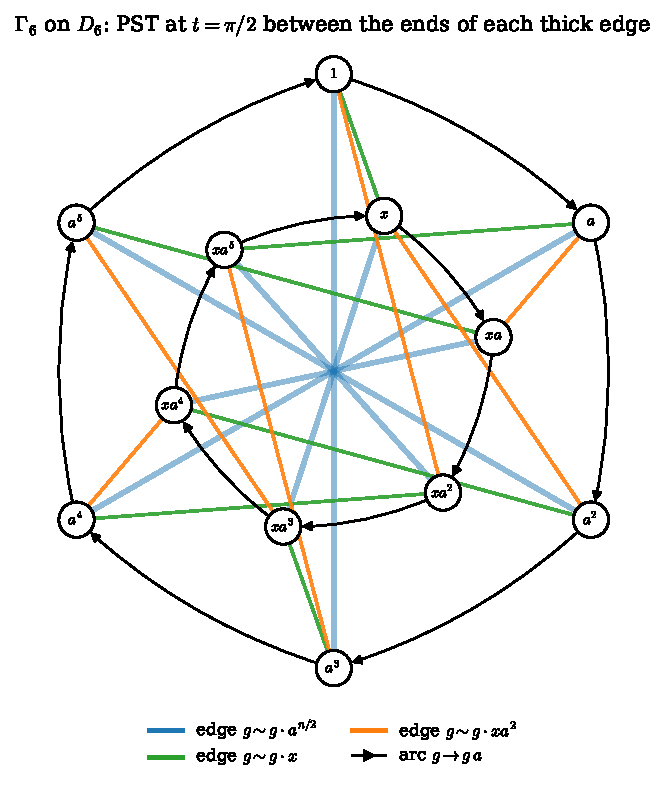
\includegraphics[trim=0 0 0 19.5bp,clip,width=\textwidth]{fig_gamma6.pdf}
\end{minipage}\hfill
\begin{minipage}[t]{0.49\textwidth}\centering
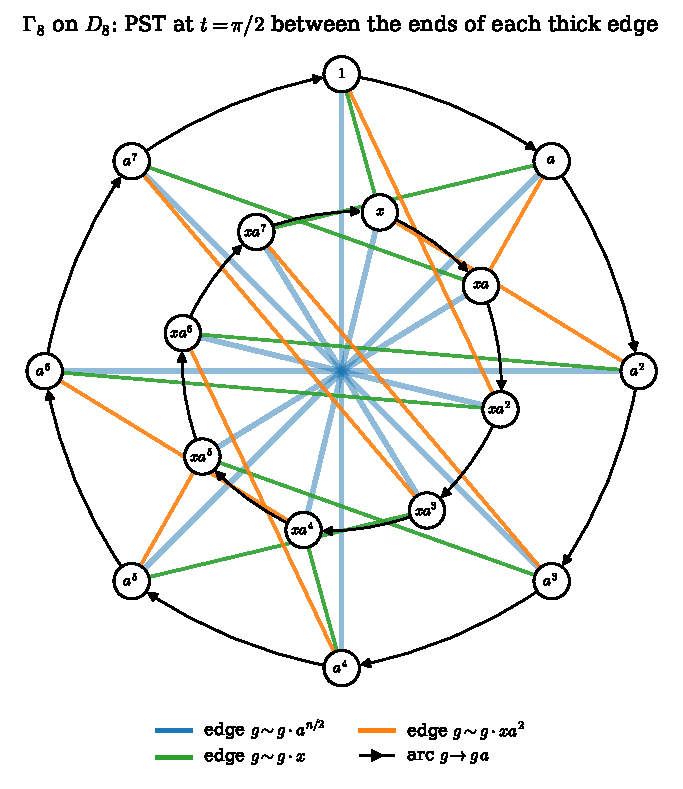
\includegraphics[trim=0 0 0 19.5bp,clip,width=\textwidth]{fig_gamma8.pdf}
\end{minipage}\\[2pt]
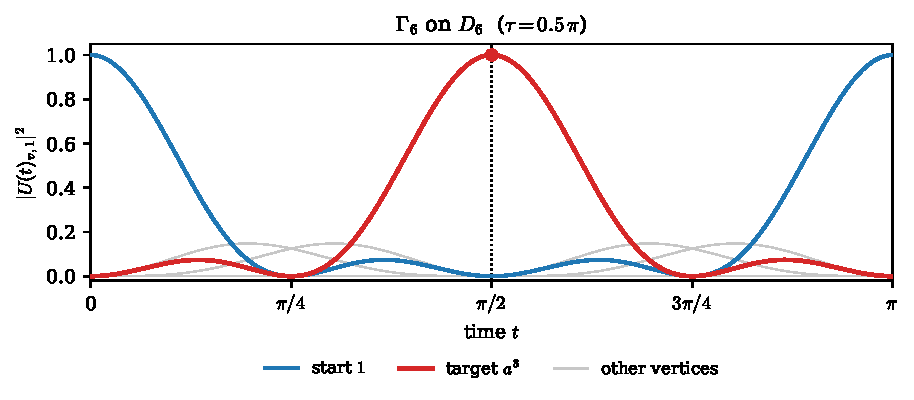
\includegraphics[trim=0 0 0 19.5bp,clip,width=0.55\textwidth]{fig_prob_gamma6.pdf}
\caption{The graphs $\Gamma_6$ and $\Gamma_8$ and the transfer probabilities for $\Gamma_6$. Top: the graphs $\Gamma_6$ and $\Gamma_8$ of Proposition~\ref{prop:Dn}: $a^k$ on the outer ring, $xa^k$ on the inner ring; thick blue edges: $g\sim ga^{n/2}$, the pairs between which PST occurs at $t=\pi/2$; green: $g\sim gx$; orange: $g\sim gxa^2$; arrows: $g\to ga$. Bottom: transfer probabilities for $\Gamma_6$; the probability at $a^3$ reaches $1$ at $t=\pi/2$ (Proposition~\ref{prop:Dn}(ii)).\label{fig:gamma}}
\end{figure}
\section{Weighing-type transfer on generalised dicyclic groups}\label{sec:gd}

\subsection{Setting and statement of the problem}

Let $A$ be a finite abelian group (written additively) and $y\in A$ with $2y=0$. The \emph{generalised dicyclic group} $G=\mathrm{Dic}(A,y)$ is the group $A\rtimes_f\Z_2$ of Section~\ref{sec:groups} with $f=-\mathrm{id}$ and $x^2=y$; thus $(a,0)(b,1)=(b-a,1)$, $(a,1)(b,0)=(a+b,1)$, $(a,1)(b,1)=(y-a+b,0)$ and
\begin{equation}\label{gd:inv}
(a,0)^{-1}=(-a,0),\qquad (a,1)^{-1}=(a+y,1).
\end{equation}
(For undirected connection sets, PST on Cayley graphs over groups with an abelian subgroup of index $2$, including generalised dihedral and generalised dicyclic groups, is characterised in~\cite{Arezoomand}; the present section concerns the mixed weighing mechanism and its classification.) For $y=0$ this is the generalised dihedral group $\mathrm{Dih}(A)$; for $A=\Z_{2n}$, $y=n$ it is $\mathrm{Dic}_n$. We assume that $A$ is not an elementary abelian $2$-group, so that $G$ is non-abelian and, by Lemma~\ref{lem:center}, $Z(G)=\Fix(-\mathrm{id})=A[2]$. The central involutions are the elements $c\in A[2]\setminus\{0\}$.

\begin{definition}\label{gd:def}
A set $S'\subseteq G\setminus\{1\}$ is a \emph{weighing set of weight $k$} if the Hermitian adjacency matrix $K$ of $\mathrm{Cay}(G,S')$ satisfies $K^2=k^2I$.
\end{definition}

By Theorem~\ref{thm:weighing}, if $k$ is even, $c\in A[2]\setminus\{0\}$ and $c\notin S'$, then $S=S'\cup\{c\}$ gives $U(\pi/2)=(-1)^{k/2+1}\ii R_c$, i.e.\ PST at time $\pi/2$ between $g$ and $gc$ for every $g$. Since $c$ enters only through the requirement $c\notin S'$ and through connectivity, \emph{the classification of PST of weighing type is the classification of weighing sets}.

\paragraph{Data of a set $S'$.} Using \eqref{gd:inv} write
\begin{align*}
P&=\{a:(a,0)\in S'\cap S'^{-1}\}, & T&=\{a:(a,0)\in S'\setminus S'^{-1}\},\\
R_u&=\{r:(r,1)\in S'\cap S'^{-1}\}, & R_a&=\{r:(r,1)\in S'\setminus S'^{-1}\}.
\end{align*}
Then $P=-P$, $T\cap(-T)=\emptyset$, $R_u=R_u+y$, and $R_a\cap(R_a+y)=\emptyset=R_a\cap R_u$. (For $y=0$ one has $R_a=\emptyset$: every element of $xA$ is an involution.) For $\psi\in\widehat A$ put
\begin{gather*}
p_\psi=\sum_{d\in P}\psi(d)\in\mathbb R,\qquad s_\psi=\sum_{t\in T}\operatorname{Im}\psi(t),\\
\beta_\psi=\sum_{r\in R_u}\overline{\psi(r)}+\ii\bigl(1-\psi(y)\bigr)\sum_{r\in R_a}\overline{\psi(r)} .
\end{gather*}
Note $\psi(y)=\pm1$. Since $R_u=R_u+y$, the first sum in $\beta_\psi$ vanishes if $\psi(y)=-1$; hence
\begin{equation}\label{gd:beta}
|\beta_\psi|=\Bigl|\sum_{r\in R_u}\psi(r)\Bigr|\ \ (\psi(y)=1),\qquad |\beta_\psi|=2\Bigl|\sum_{r\in R_a}\psi(r)\Bigr|\ \ (\psi(y)=-1).
\end{equation}

\subsection{A complete Fourier criterion for every weight}

\begin{theorem}[Criterion and dichotomy]\label{gd:fourier}
Let $S'\subseteq G\setminus\{1\}$ and $k\ge1$.
\begin{enumerate}
\item[(a)] $K^2=k^2I$ if and only if for every $\psi\in\widehat A$
\begin{equation}\label{gd:F}
p_\psi s_\psi=0,\qquad p_\psi\beta_\psi=0,\qquad (p_\psi+2s_\psi)^2+|\beta_\psi|^2=k^2 .
\end{equation}
\item[(b)] If $K^2=k^2I$, then exactly one of the following holds: \emph{Type~I}: $P=\emptyset$ and $|R_u|=k$; \emph{Type~II}: $R_u=\emptyset$ and $|P|=k$. In both cases $|T|+|R_a|=k(k-1)/2$. If $y=0$ and $\langle S'\cup\{c\}\rangle=G$, then $S'$ has Type~I.
\item[(c)] A set of Type~I has weight $k$ if and only if $P=\emptyset$, $|R_u|=k$, $|T|+|R_a|=k(k-1)/2$ and
\begin{align}
&4s_\psi^2+\Bigl|\sum_{r\in R_u}\psi(r)\Bigr|^2=k^2 &&\text{for all }\psi\text{ with }\psi(y)=1,\tag{E1}\\
&4s_\psi^2+4\Bigl|\sum_{r\in R_a}\psi(r)\Bigr|^2=k^2 &&\text{for all }\psi\text{ with }\psi(y)=-1.\tag{E2}
\end{align}
(For $y=0$ only (E1) occurs.)
\item[(d)] A set of Type~II has weight $k$ if and only if $R_u=\emptyset$, $|P|=k$, $|T|+|R_a|=k(k-1)/2$ and, for all $\psi$: $p_\psi s_\psi=0$; $(p_\psi+2s_\psi)^2=k^2$ if $\psi(y)=1$; $p_\psi\sum_{R_a}\psi=0$ and $(p_\psi+2s_\psi)^2+4|\sum_{R_a}\psi|^2=k^2$ if $\psi(y)=-1$.
\end{enumerate}
\end{theorem}

\begin{proof}
Apply Theorem~\ref{thm:N}(a) to $\mathrm{Cay}(G,S')$. Here $h_0=1$ on $P$, $h_0=\ii$ on $T$, $h_0=-\ii$ on $-T$, and $h_1=1$ on $R_u$, $h_1=\ii$ on $R_a$, $h_1=-\ii$ on $R_a+y$. Hence $\alpha_\psi=p_\psi+2s_\psi$, and since $\psi^f=\overline\psi$ we get $\alpha_{\psi^f}=p_\psi-2s_\psi$, while $\beta_\psi$ is as defined above (use $\overline{\psi(r+y)}=\psi(y)\overline{\psi(r)}$). As $\psi(y)$ is real,
\begin{gather*}
M_\psi=\begin{pmatrix}p_\psi+2s_\psi&\psi(y)\overline{\beta_\psi}\\ \psi(y)\beta_\psi&p_\psi-2s_\psi\end{pmatrix},\\
M_\psi^2=\begin{pmatrix}(p+2s)^2+|\beta|^2&2p\,\psi(y)\overline{\beta}\\ 2p\,\psi(y)\beta&(p-2s)^2+|\beta|^2\end{pmatrix}.
\end{gather*}
Now $K^2=k^2I$ holds if and only if $M_\psi^2=k^2I_2$ for all $\psi$, that is, if and only if $p\beta=0$ and $(p\pm2s)^2+|\beta|^2=k^2$; subtracting the last two equations gives $8ps=0$, so the system is equivalent to \eqref{gd:F}. This proves the first assertion.

For the dichotomy, take $\psi=1$: then $s_1=0$, $p_1=|P|$ and $\beta_1=|R_u|$, so \eqref{gd:F} gives $|P||R_u|=0$ and $|P|^2+|R_u|^2=k^2$, which means that either $P=\emptyset$ and $|R_u|=k$, or $R_u=\emptyset$ and $|P|=k$. The diagonal of $K^2$ equals the number of non-zero entries in a row, namely $|P|+2|T|+|R_u|+2|R_a|=k^2$, and since $|P|+|R_u|=k$ this yields $|T|+|R_a|=k(k-1)/2$. If $y=0$, then $R_a=\emptyset$, so Type~II would force $S'\cup\{c\}\subseteq A$, which does not generate $G$; thus $S'$ has Type~I. Finally, the descriptions of Type~I and Type~II sets are the first assertion specialised to $P=\emptyset$, respectively $R_u=\emptyset$, combined with \eqref{gd:beta}.
\end{proof}

Theorem~\ref{gd:fourier} is an exact description for \emph{all} weights; it contains Lemma~\SR{lem:kgen} (the case $y=0$, where (E1) is the identity $|\sum_R\psi|^2+(2\sum_T\operatorname{Im}\psi)^2=k^2$).

\subsection{Weight $2$: complete classification}

\begin{theorem}[Weight $2$]\label{gd:k2}
Let $G=\mathrm{Dic}(A,y)$ be non-abelian, $c\in A[2]\setminus\{0\}$, and let $S'\subseteq G\setminus\{1\}$ with $c\notin S'$ and $\langle S'\cup\{c\}\rangle=G$. Then $K^2=4I$ if and only if $S'$ is one of the following.
\begin{enumerate}
\item[(B1)] ($y=0$) $S'=\{(r,1),(r+2t,1),(t,0)\}$ with $r,t\in A$, $2t\ne0$; connected iff $A=\langle c,t\rangle$.
\item[(B2a)] ($y\ne0$) $S'=\{(r,1),(r+y,1),(t,0)\}$ with $2t=y$; connected iff $A=\langle c,t\rangle$.
\item[(B2b)] ($y\ne0$) $S'=\{(r,1),(r+y,1),(u,1)\}$ with $u\notin\{r,r+y\}$; connected iff $A=\langle c,y,u-r\rangle$.
\item[(B3)] ($y\ne0$) $S'=\{(d,0),(-d,0),(u,1)\}$ with $2d=y$; connected iff $A=\langle c,d\rangle$.
\end{enumerate}
In (B1), (B2a), (B2b) $S'$ has Type~I, in (B3) Type~II (the latter forces $A=\langle c,d\rangle$ with $d$ of order $4$, so $|A:A[2]|\le2$ and $G$ has a second abelian subgroup of index $2$). In (B1)--(B2b), $(r,1),(r+2t,1)$ (resp.\ $(r,1),(r+y,1)$) are undirected edges; $(t,0)$ and $(u,1)$ are arcs. In all cases $U(\pi/2)=\ii R_c$.
\end{theorem}

\begin{proof}
By Theorem~\ref{gd:fourier}(b) with $k=2$, either $|R_u|=2$ and $P=\emptyset$ (Type~I), or $|P|=2$ and $R_u=\emptyset$ (Type~II), and in both cases $|T|+|R_a|=1$.

Consider first Type~I with $y=0$. Then $R_a=\emptyset$, $T=\{t\}$ and $R_u=\{r,r'\}$; put $d=r'-r$. Condition (E1) reads $2+2\operatorname{Re}\psi(d)+4(\operatorname{Im}\psi(t))^2=4$, that is, $\operatorname{Re}\psi(d)=\operatorname{Re}\psi(2t)$ for all $\psi$, and by Fourier inversion $\{d,-d\}=\{2t,-2t\}$. Thus $r'=r\pm2t$, and the set $\{r,r-2t\}$ is of the form $\{r'',r''+2t\}$ with $r''=r-2t$; moreover $2t\ne0$ because $T\cap(-T)=\emptyset$. This is (B1).

For Type~I with $y\ne0$ we have $R_u=\{r,r+y\}$, so $|\sum_{R_u}\psi|=2$ whenever $\psi(y)=1$. If $T=\{t\}$ and $R_a=\emptyset$, then (E1) forces $\operatorname{Im}\psi(t)=0$, that is $\psi(2t)=1$, for all $\psi$ with $\psi(y)=1$; hence $2t\in\langle y\rangle$, and $2t\ne0$ gives $2t=y$. For $\psi(y)=-1$ we then have $\psi(t)=\pm\ii$, and (E2) reads $4=4$. This is (B2a). If instead $T=\emptyset$ and $R_a=\{u\}$, both (E1) and (E2) read $4=4$, and admissibility requires only $u\notin R_u$; this is (B2b).

In Type~II, connectivity needs $R_a\ne\emptyset$ (otherwise $S'\cup\{c\}\subseteq A$), so $R_a=\{u\}$, $T=\emptyset$, $s_\psi\equiv0$ and $P=\{d,e\}$. By Theorem~\ref{gd:fourier}(d), for $\psi(y)=1$ we need $|\psi(d)+\psi(e)|=2$, that is $\psi(d)=\psi(e)$, and for $\psi(y)=-1$ we need $p_\psi=0$, that is $\psi(e)=-\psi(d)$. Hence $\psi(e-d)=\psi(y)$ for all $\psi$, so $e=d+y$, and $P=-P$ then gives $2d\in\{0,y\}$. If $2d=0$, then $\langle S'\cup\{c\}\rangle\cap A\subseteq A[2]$ and the generated group is abelian, which is excluded; so $2d=y$ and $P=\{d,-d\}$, which is (B3).

The connectivity conditions follow from~\eqref{gd:inv}: in (B1), $(r,1)(r+2t,1)=(2t,0)$; in (B2a), $(r,1)^{-1}(r+y,1)=(y,0)$; in (B2b), $(r,1)^{-1}(u,1)=(u-r,0)$ and $(r,1)^2=(y,0)$; in (B3), $(u,1)^2=(y,0)=(2d,0)$. In each case the subgroup generated by $S'\cup\{c\}$ consists of a subgroup $H_0\le A$, namely the one stated in the theorem, together with the coset of $H_0$ by an element outside $A$. The last assertion of the theorem is Theorem~\ref{thm:weighing}.
\end{proof}

\begin{remark}
(B1) with $A=\Z_n$ is Proposition~\ref{prop:Dn}. (B2b) with $y=c$ is the family of Proposition~\SR{prop:dic}; no relation between $c$ and $y$ is needed, and (B2a), (B3) are not contained in Proposition~\SR{prop:dic}. Theorem~\ref{gd:k2} was checked against an exhaustive search over all subsets $S'$ with $|S'|\in\{2,3,4\}$ (the possible sizes when $|S'\cup S'^{-1}|=4$), in exact integer arithmetic, for every cyclic $A=\Z_m$ with $3\le m\le24$ and for $A\in\{\Z_4\times\Z_2,\Z_6\times\Z_2,\Z_8\times\Z_2,\Z_4^2,\Z_{10}\times\Z_2,\Z_{12}\times\Z_2,\Z_4\times\Z_2^2,\Z_6\times\Z_4,\Z_3^2\}$, for all $y\in A[2]$ and all $c\in A[2]\setminus\{0\}$ (162 triples $(A,y,c)$): the sets of connected pairs $(S',c)$ coincide with the union of (B1)--(B3) in every case.
\end{remark}

\subsection{Weight $4$: an infinite family on $\mathrm{Dic}(A,y)$ with $y\neq0$}

For $y=0$ our searches found no weight-$4$ example on a cyclic $A$ (Remark~\SR{rem:kgen}(iii)); Theorem~\ref{gd:fourier} shows why the mechanism below is unavailable there: it needs arcs in $xA$ and the pairing $\{t,y-t\}$.

\begin{proposition}[Weight $4$ for $y\neq0$]\label{gd:k4}
Let $y\in A[2]\setminus\{0\}$ and $\rho,u,a\in A$. Put
\begin{align*}
R_u&=\{0,\,y,\,2\rho,\,2\rho+y\},\qquad T=\{\rho,\ \rho+y,\ u,\ y-u\},\\
R_a&=\{a,\ a+2u\},\\
S'&=\{(r,1):r\in R_u\}\ \cup\ \{(t,0):t\in T\}\ \cup\ \{(r,1):r\in R_a\},
\end{align*}
where $(r,1)$, $r\in R_u$, are undirected and the other six elements are arcs. Assume that $2\rho\notin\{0,y\}$; that the elements of $T$ are distinct and $T\cap(-T)=\emptyset$; that $2u\notin\{0,y\}$; and that $a,a+2u\notin R_u$. Then $K^2=16I$. Consequently, for every $c\in A[2]\setminus\{0\}$, $\mathrm{Cay}(G,S'\cup\{c\})$ has PST at time $\pi/2$ with $U(\pi/2)=-\ii R_c$, spectrum contained in $\{\pm3,\pm5\}$, and it is connected iff $A=\langle c,y,\rho,u,a\rangle$. If moreover $4\rho\notin\{0,y\}$, it is not isomorphic to a mixed Cayley graph of any abelian group.
\end{proposition}

\begin{proof}
The assumptions say exactly that $S'$ is admissible with data $P=\emptyset$, $|R_u|=4$ and $|T|+|R_a|=6$, so $S'$ is of Type~I with $k=4$, and it suffices to verify (E1) and (E2). Write $\psi(\rho)=\exp\bigl(\ii\theta\bigr)$ and $\psi(u)=\exp\bigl(\ii\varphi\bigr)$. If $\psi(y)=1$, then $\psi(y-u)=\overline{\psi(u)}$, so $s_\psi=2\operatorname{Im}\psi(\rho)=2\sin\theta$ and $|\sum_{R_u}\psi|=|(1+\psi(y))(1+\psi(2\rho))|=2|1+\exp\bigl(2\ii\theta\bigr)|=4|\cos\theta|$; hence $4s_\psi^2+|\sum_{R_u}\psi|^2=16\sin^2\theta+16\cos^2\theta=16$. If $\psi(y)=-1$, then $\operatorname{Im}\psi(\rho+y)=-\operatorname{Im}\psi(\rho)$ and $\psi(y-u)=-\overline{\psi(u)}$, so $s_\psi=2\operatorname{Im}\psi(u)=2\sin\varphi$ and $|\sum_{R_a}\psi|=|1+\psi(2u)|=2|\cos\varphi|$; hence $4s_\psi^2+4|\sum_{R_a}\psi|^2=16\sin^2\varphi+16\cos^2\varphi=16$. By Theorem~\ref{gd:fourier}(c), $K^2=16I$, and Theorem~\ref{thm:weighing} gives $U(\pi/2)=(-1)^{4/2+1}\ii R_c=-\ii R_c$. On the block of $\psi$ the matrix $H=L_c+K$ has the eigenvalues $\psi(c)\pm4$, which accounts for the stated spectrum. For connectivity, $(0,1)^{-1}(r,1)=(r,0)$ for $r\in R_u\cup R_a$, so $\langle S'\cup\{c\}\rangle\cap A=\langle c,y,\rho,u,a\rangle$, and the group generated is this subgroup together with $(0,1)$.

To prove the last assertion, we apply Lemma~\ref{lem:abtest}: it suffices to show that $\sum_{s\in S_u,t\in T_{\rm all}}(\rho(ts)-\rho(st))\ne0$. The terms with $s=c$ cancel because $c$ is central, and the terms with $t\in xA$ lie in $A$, so they cannot cancel terms in $xA$. For $t\in A$ and $s=(r,1)$ we have $(t,0)(r,1)=(r-t,1)$ and $(r,1)(t,0)=(r+t,1)$. In $\Z[A]$ (written multiplicatively) the $xA$-component of the sum is therefore $R_u\,(T^{(-1)}-T)$, with $R_u=(1+y)(1+\rho^2)$ and $T=\rho(1+y)+u+yu^{-1}$. Since $(1+y)(1-y)=0$, the $u$-part drops out and
\[
R_u(T^{(-1)}-T)=(1+y)^2(1+\rho^2)(\rho^{-1}-\rho)=2(1+y)(\rho^{-1}-\rho^{3}),
\]
which is non-zero if and only if $\rho^{-1}\notin\{\rho^3,y\rho^3\}$, that is, if and only if $4\rho\notin\{0,y\}$.
\end{proof}

\begin{corollary}[$\mathrm{Dic}_n$, $n\ge5$]\label{gd:dicn}
Let $n\ge5$, $A=\Z_{2n}$, $y=c=n$, $\rho=1$, $u=2$, so $R_u=\{0,n,2,n+2\}$, $T=\{1,2,n-2,n+1\}$, $R_a=\{a,a+4\}$ with $a=1$ ($n\ge6$) or $a=4$ ($n=5$). Then $\mathrm{Cay}(\mathrm{Dic}_n,S'\cup\{n\})$ is connected, has $\zeta=5$, $K^2=16I$, PST at time $\pi/2$ with $U(\pi/2)=-\ii R_c$, and is not a Cayley graph of any abelian group. For $n\in\{3,4\}$ there is no weighing set of weight $4$ at all: the diagonal of $K^2=16I$ forces $|S'\cup S'^{-1}|=16$, whereas $S'\cup S'^{-1}\subseteq G\setminus\{1,c\}$ has at most $4n-2\le14$ elements.
\end{corollary}

\begin{proof}
The hypotheses of Proposition~\ref{gd:k4} are checked directly: for $n\ge5$ the four elements of $T$ are distinct, none is the negative of another, $2\rho=2\notin\{0,n\}$, $2u=4\notin\{0,n\}$ (as $n\ne4$), $4\rho=4\notin\{0,n\}$, and $a,a+4\notin R_u$ for the stated $a$. $A=\langle1\rangle$, so $S'\cup\{c\}$ generates. The last statement for $n=3,4$ follows from the counting argument stated above (it is also confirmed by the exhaustive enumeration of Section~\ref{sec:gd-comp}).
\end{proof}

\subsection{Computations and what is not classified}\label{sec:gd-comp}

\begin{remark}[Computational facts, weight $4$]
All searches here use integer arithmetic only. Theorem~\ref{gd:fourier}(b) restricts the shape of $S'$ (undirected part of weight $4$ in $xA$ (Type~I) or in $A$ (Type~II), arc part of weight $12$); we enumerated all weighing sets of weight $4$ on $\mathrm{Dic}(A,y)$, testing each candidate by $\kappa*\kappa=16\delta$ and then $K^2=16I$, together with connectivity, for all abelian $A$ of order $\le16$ that are not elementary abelian and all $y\in A[2]$. On $\mathrm{Dic}_n$ ($y=n$) there is none for $n\le4$, and the enumeration finds exactly $80,\,288,\,1176,\,2688,\,4320$ sets for $n=5,\dots,9$, all of Type~I and connected. For $n\ge10$ existence follows from Corollary~\ref{gd:dicn}, whose conclusion $K^2=16I$ was verified by computer for $5\le n\le60$ ($K^2=16I$ in integer arithmetic). On $\Z_{2n}$ with $y=0$ (dihedral groups of order $4n$) there is none for $2n\le34$, in agreement with Remark~\SR{rem:kgen}(iii). For non-cyclic $A$ with $y\ne0$ and $|A|\le16$, connected sets exist for $\Z_6\times\Z_2$, $\Z_8\times\Z_2$, $\Z_4^2$ and $\Z_4\times\Z_2^2$ (all $y\ne0$ except $y=(2,0,0)$) and do not exist for $\Z_8$ and $\Z_4\times\Z_2$; for $y=0$ only $\Z_4^2$ (of the groups listed) has one. Type~II sets of weight $4$ occur, for example for $\Z_4^2$ and $\Z_8\times\Z_2$ with $y\ne0$.

\emph{Cross-checks.} No weighing set of weight $4$ exists when $|G|<18$ (counting argument of Corollary~\ref{gd:dicn}); this covers $\mathrm{Dic}_3$, $\mathrm{Dic}_4$ and all groups $\mathrm{Dic}(A,y)$ of order $16$. Enumerations over all subsets $S'\subseteq G\setminus\{1,c\}$, filtered only by the necessary condition that every row of $K$ has $16$ non-zero entries, give the counts $0,0,80,288$ on $\mathrm{Dic}_3,\dots,\mathrm{Dic}_6$, and an enumeration pruned only by $|S'\cap S'^{-1}|=4$ and $|S'\setminus S'^{-1}|=6$ (both consequences of $K^2=16I$) gives $1176$ on $\mathrm{Dic}_7$; all tests are exact (integer arithmetic). The restricted enumeration of Theorem~\ref{gd:fourier}(b) agrees with these counts. The family of Proposition~\ref{gd:k4} was verified by computer for $\mathrm{Dic}_n$, $5\le n\le60$ ($K^2=16I$ in integer arithmetic). For $y\ne0$ we make no non-existence claim for $|A|>16$. The counts are computational evidence, not a formally verified proof.
\end{remark}

\begin{remark}[Scope]
Theorem~\ref{gd:fourier} reduces weighing-type transfer, for every $k$, to the identities (E1), (E2) (resp.\ their Type~II analogues) for subsets of $A$; this is an exact criterion, not a list. A list is obtained for $k=2$ (Theorem~\ref{gd:k2}). For $k=4$ we give an infinite family (Proposition~\ref{gd:k4}) that does not exhaust the weight-$4$ sets: on $\mathrm{Dic}_7$ the search finds sets outside this parameter pattern. Whether weight $4$ is impossible on every dihedral group is open.
\end{remark}

\section{Open problems}\label{sec:open}

\emph{Scope of the results.} The explicit examples of this paper come from one mechanism, transfer at time $\pi/2$ through a central involution $c\in S$ (Theorem~\ref{thm:pi2}), on groups $A\rtimes_f\Z_2$; Theorems~\ref{thm:G} and~\ref{thm:B} concern arbitrary connection sets, but the paper does not decide whether other mechanisms give mixed PST graphs without an abelian Cayley presentation, and it says nothing about undirected graphs beyond Remark~\ref{rem:mixedonly}. Assertions that no abelian group acts regularly rest on the sufficient test of Lemma~\ref{lem:abtest} (and on $\mathrm{Aut}=L(G)$ for $\Gamma_n$).

\begin{enumerate}
\item \textbf{Beyond weighing sets.} Theorem~\ref{thm:pi2} allows any spectrum of $K$ inside one residue class modulo $4$. Enumerating all connection sets of the groups of order at most $16$ gives connected graphs with $c\in\langle S'\rangle$ and at least three distinct eigenvalues of $K$ on $D_4$, $Q_8$, $D_6$, $\mathrm{Dic}_3$ and on each of the nine groups of order $16$ (for $D_8$ and $Q_{16}$: $78$ and $334$ sets), and none on $S_3$, $D_5$, $D_7$. Classify the sets of this kind on $A\rtimes_f\Z_2$, and decide which of them are not abelian Cayley graphs.
\item \textbf{Weight $4$ on dihedral groups.} Is the identity $RR^{(-1)}+DD^{(-1)}=16$ of Remark~\SR{rem:kgen}(v) unsolvable in $\Z[A]$ for every cyclic $A$, that is, is there no weight-$4$ set on any $D_n$, as the search for $n\le34$ suggests? Classify the weight-$4$ sets on $\mathrm{Dic}(A,y)$ (Theorem~\ref{gd:fourier} reduces this to (E1), (E2)), and decide whether weights $k>4$ occur for $y\ne0$.
\item \textbf{Undirected graphical regular representations.} Are there infinitely many graphical regular representations of non-abelian groups with PST \cite[Problem~8.2]{AG}? Proposition~\ref{prop:Dn} answers only the mixed analogue, and the weighing mechanism cannot give undirected examples (Remark~\ref{rem:mixedonly}). By Remark~\ref{rem:toggle}, PST at time $\pi/2$ through a central involution $c$ asks for an undirected connection set $S^\circ$ such that $\mathrm{Cay}(G,S^\circ)$ has all eigenvalues congruent to its valency modulo $4$ and $\mathrm{Cay}(G,S^\circ\,\triangle\,\{c\})$ is a graphical regular representation; the $32$-vertex example of \cite[Section~6.1]{AG}, where the transfer time is $\pi/2$, is of this form with $c\notin S$. Find such sets in an infinite family.
\item \textbf{Targets of order $4$ for non-normal sets.} For $f=-\mathrm{id}$ and non-normal $S$, targets of order $4$ occur (Table~\ref{tab:nn}), although normal sets forbid them. Describe the connection sets with such targets.
\item \textbf{The case $\zeta=0$ and the parity condition.} For $\zeta=0$ order $3$ occurs and order $6$ is not excluded \cite{CPRS}, and Theorem~\ref{thm:G}(b) fails. For undirected graphs a non-abelian group with an abelian subgroup of index $2$ has a connected Cayley graph with PST if and only if $4\mid|G|$ \cite{AG}; does the same hold for connected mixed Cayley graphs with $\zeta>0$? The mixed sets with $\zeta>0$ on $\Z_n$, $n=6,10,14$, support this.
\item \textbf{Automorphism groups of the dicyclic family.} For the graphs of Proposition~\SR{prop:dic} on $\mathrm{Dic}_n$ we computed $|\Aut|=n\,2^{n+1}$ for $3\le n\le10$ (Remark~\SR{rem:dic}(i)). Does this formula hold for all $n\ge3$? What are $\Aut$ for $n\ge8$ and for $SD_{2^k}$, and is any member a graphical regular representation in the mixed sense?
\end{enumerate}


\section*{Data availability}
The verification archive for this paper is available at \textbf{\ArchiveLink}. It contains the author's scripts with the logs they produced (directory \texttt{author\_scripts\_original}) and a second, independently written set of programs with their logs (directory \texttt{independent\_checks}, with \texttt{README}, \texttt{run\_all.sh} and \texttt{requirements.txt}; Python 3.12.3, numpy 2.4.4, scipy 1.17.1, pynauty 2.8.8.1). The two \texttt{README} files state, for each group of computed statements, the script that produces it. Together the scripts reproduce: the identities, the connectivity and the commutation test of Lemma~\ref{lem:abtest} for the families of Propositions~\ref{prop:Dn}, \SR{prop:dic}, \SR{prop:k4fam} and Corollary~\ref{gd:dicn} on the parameter ranges stated there (double precision; for Corollary~\ref{gd:dicn} also exactly, for $5\le n\le60$); the counts $0,0,80,288,1176$ of weight-$4$ weighing sets on $\mathrm{Dic}_3,\dots,\mathrm{Dic}_7$ by enumerations over all subsets in exact integer arithmetic, one of them pruned only by $|S'\cap S'^{-1}|=4$ and $|S'\setminus S'^{-1}|=6$, which follow from $K^2=16I$ alone, and the counts $2688,4320$ on $\mathrm{Dic}_8,\mathrm{Dic}_9$ (by an enumeration restricted with Theorem~\ref{gd:fourier}(b), hence not independent of that theorem); the exhaustive check of Theorem~\ref{gd:k2} over the $162$ triples $(A,y,c)$ in exact integer arithmetic; Tables~\ref{tab:nn} and~\ref{tab:ab} for all groups of order at most $16$, including the target columns and the per-group $|\Aut|$ column, computed by the author's program in double precision and by an independent program with the exact certification described in Appendix~\ref{sec:comp} (the two give identical tables); Table~\SR{tab:normal}; the automorphism orders of the families of Proposition~\ref{prop:Dn} ($n=6,8,10,12$; also up to $n=16$ in the independent programs); the family of Proposition~\SR{prop:k4fam} for $2\le m\le10$ (exact $K^2=16I$, transfer matrix, commutation test and $|\mathrm{Aut}|$; the commutation test vanishes for $m=2$, where $|\mathrm{Aut}|=6144$); the abelian-regular-subgroup cross-check of Table~\ref{tab:ab} and of Remark~\SR{rem:dic} (computed by backtracking and, independently, with \texttt{nauty}); the enumeration of the weight-$4$ weighing sets on $\mathrm{Dic}(A,y)$ for the non-cyclic groups $A$ of order at most $16$ and all $y\in A[2]$ (exact integer arithmetic; the pruning to four undirected elements and six arcs, a consequence of $K^2=16I$, is validated against the row-count-only enumeration on $\Z_6\times\Z_2$); the absence of weight-$4$ solutions on cyclic $A$ for $13\le n\le34$, by the author's search (rounded floating-point keys) and by an independent exact search (integer autocorrelation keys) with a positive control on $\Z_4\times\Z_8$ ($1008$ solutions); the claim on $\Z_n$, $n=6,10,14$; the counts $78$ and $334$ of Open problem~1; and Lemma~\SR{lem:Cn} and the multiple state transfer family of Proposition~\SR{prop:mst} for $5\le n\le8$. Floating-point arithmetic is used elsewhere (spectra, block decomposition of Theorem~\ref{thm:N}, the families above) with tolerances between $10^{-6}$ and $10^{-9}$; those results are numerical evidence, not proofs. The archive does not contain a formal proof-checker verification of any theorem.

\section*{Declaration of generative AI and AI-assisted technologies in the manuscript preparation process}
During the preparation of this work the author(s) used Claude (Anthropic) in order to review the manuscript as a referee, to check proofs and numerical claims, to write and run verification code for the computations reported in Appendices~\ref{sec:search} and~\ref{sec:comp} and in the supplementary note, and to edit the \LaTeX{} source. After using this tool, the author(s) reviewed and edited the content as needed and take(s) full responsibility for the content of the publication.

% ---- Elsevier declarations: UNCOMMENT AND COMPLETE ONLY IF THE STATEMENT IS TRUE (check the Guide for Authors of the journal) ----
% \section*{Declaration of competing interest}
% (state truthfully whether there are competing interests)
% \section*{Funding}
% (state the funding sources, or that there is none)
% \section*{CRediT authorship contribution statement}
% (if requested: roles of each author)

\appendix

\section{Proof of the structure theorem}\label{app:G}

\begin{proof}[Proof of Theorem~\ref{thm:G}]
Write $U=U(t)$, and for $g\in\mathrm{Aut}(\Gamma)$ let $Q_g$ be its permutation matrix; $Q_g$ commutes with $H$ and hence with every $U(t)$. By transitivity all out-degrees equal a common value $d^+$ and all in-degrees a common value $d^-$, and counting arcs gives $d^+=d^-$. Every row sum of $H$ is therefore $\zeta+\ii d^+-\ii d^-=\zeta$; that is, $H\mathbf 1=\zeta\mathbf 1$ and $U(t)\mathbf 1=\exp\bigl(-\ii t\zeta\bigr)\mathbf 1$ for all $t$.

Now let $t>0$ and suppose that $Ue_u=\lambda e_w$ for some vertex $w$ (possibly $w=u$) and some $|\lambda|=1$; since $U$ is unitary, this holds whenever $|U_{w,u}|=1$. PST from $u$ to $v$ at time $\tau$ is the case $t=\tau$, $w=v\ne u$, and periodicity at $u$ is the case $w=u$. For any vertex $w'$ choose $g\in\mathrm{Aut}(\Gamma)$ with $g(u)=w'$; then $Ue_{w'}=UQ_ge_u=Q_gUe_u=\lambda e_{g(w)}$. The left-hand side does not depend on the choice of $g$, so $g(w)$ depends only on $w'$, and we may put $\sigma(w')=g(w)$. Thus $Ue_{w'}=\lambda e_{\sigma(w')}$ for every vertex $w'$, and since the columns of $U$ are orthonormal, $\sigma$ is injective, hence a permutation, with $U=\lambda P_\sigma$ and $\sigma(u)=w$. For $g\in\mathrm{Aut}(\Gamma)$ the relation $UQ_g=Q_gU$ gives $\lambda e_{\sigma(g(x))}=\lambda e_{g(\sigma(x))}$, so $\sigma g=g\sigma$; moreover $P_\sigma=\lambda^{-1}U$ commutes with $H$, so $\sigma$ preserves edges and arcs. Hence $\sigma\in\mathrm{Aut}(\Gamma)$ and therefore $\sigma\in Z(\mathrm{Aut}(\Gamma))$. If $w=u$, then for every vertex $x=g(u)$ we get $\sigma(x)=g(\sigma(u))=g(u)=x$, so $\sigma=\mathrm{id}$. If $w\ne u$ and $\sigma(y)=y$ for some vertex $y$, then choosing $g$ with $g(y)=u$ we would get $\sigma(u)=g(\sigma(y))=u\ne w$, a contradiction; so $\sigma$ is fixed-point-free whenever $w\ne u$. Comparing $P_\sigma\mathbf 1=\mathbf 1$ with $U\mathbf 1=\exp\bigl(-\ii t\zeta\bigr)\mathbf 1$ shows that $\lambda=\exp\bigl(-\ii t\zeta\bigr)$. This proves the first part of (a), and also that $U(t)=\exp\bigl(-\ii t\zeta\bigr)I$ when $w=u$.

Integrality of the spectrum is the next consequence. Put $P=P_\sigma$ and $d=\ord(\sigma)$, with $d=1$ if $w=u$, so that $P^d=I$. On the eigenspace $V_\theta$ of an eigenvalue $\theta$ of $H$ we have $U=\exp\bigl(-\ii t\theta\bigr)I$, so $P=\lambda^{-1}U$ acts on $V_\theta$ as the scalar $\omega_\theta=\exp\bigl(-\ii t\theta\bigr)/\lambda=\exp\bigl(-\ii t(\theta-\zeta)\bigr)$, and $\omega_\theta^d=1$. Hence $t(\theta-\theta')\in2\pi\Q$ for all eigenvalues $\theta,\theta'$. Since $\zeta$ is itself an eigenvalue, with eigenvector $\mathbf 1$, this means $\theta=\zeta+\kappa q_\theta$ with $\kappa=2\pi/t>0$ and $q_\theta\in\Q$. Let $m_\theta$ be the multiplicities and $n$ the number of vertices. As $\mathrm{tr}\,H=0$, we have $0=n\zeta+\kappa\sum_\theta m_\theta q_\theta$; because $\zeta>0$ the sum $\sum_\theta m_\theta q_\theta$ is non-zero, and $\kappa=-n\zeta/\sum_\theta m_\theta q_\theta\in\Q$. Thus every $\theta$ is rational, and being an algebraic integer (a root of the characteristic polynomial of a matrix over $\Z[\ii]$), it is an integer; also $t=2\pi/\kappa\in2\pi\Q$. This proves (b), and shows that (i) implies (iii) in~(P).

The remaining implications in~(P) are now short. If $\Gamma$ is periodic at $u$, we are in the case $w=u$ above, so $\sigma=\mathrm{id}$ and $U(t)=\exp\bigl(-\ii t\zeta\bigr)I$ is scalar; this is (i)$\Rightarrow$(ii), while (ii)$\Rightarrow$(i) is trivial. For (iii)$\Rightarrow$(ii), note that not all eigenvalues equal $\zeta$, since $H$ has zero diagonal and $\zeta>0$; so $\gamma$ is a positive integer, every $\theta-\zeta$ lies in $\gamma\Z$, and hence $U(2\pi k/\gamma)=\exp\bigl(-2\pi\ii k\zeta/\gamma\bigr)I$. Conversely, if $U(t)$ is scalar, then $t(\theta-\zeta)\in2\pi\Z$ for all $\theta$, because $U(t)\mathbf 1=\exp\bigl(-\ii t\zeta\bigr)\mathbf 1$, and a B\'ezout combination of the integers $\theta-\zeta$ gives $t\gamma\in2\pi\Z$. So $U(t)$ is scalar exactly for $t\in(2\pi/\gamma)\Z$.

To bound the order of $\sigma$, observe that by (b) the spectral idempotents $E_\theta=\prod_{\theta'\ne\theta}(H-\theta'I)/(\theta-\theta')$ have entries in $\Q(\ii)$. From $PE_\theta=\omega_\theta E_\theta$ and $E_\theta\ne0$ we may choose an entry $(a,b)$ with $(E_\theta)_{ab}\ne0$ and conclude $\omega_\theta=(PE_\theta)_{ab}/(E_\theta)_{ab}\in\Q(\ii)$, since $P$ has integer entries. The only roots of unity in $\Q(\ii)$ are $\pm1,\pm\ii$, so $\omega_\theta^4=1$ for every $\theta$, and $P^4=\sum_\theta P^4E_\theta=\sum_\theta E_\theta=I$; that is, $\sigma^4=1$. As $\sigma$ is fixed-point-free, $\ord(\sigma)\in\{2,4\}$. If $\Gamma$ is undirected, then $H$ is real symmetric, so $U$ and hence $P_\sigma$ are symmetric; then $P_\sigma=P_\sigma^\top=P_\sigma^{-1}$ and $\sigma^2=1$. A fixed-point-free permutation of order dividing $4$ has only cycles of length $2$ and $4$, so the number of vertices is even. This is (c).

The same relation $\omega_\theta^4=1$ determines the possible transfer times. It gives $4\tau(\theta-\zeta)\in2\pi\Z$ for all $\theta$, and a B\'ezout combination of the integers $\theta-\zeta$ yields $4\tau\gamma\in2\pi\Z$, that is, $\tau=\pi\ell/(2\gamma)$ with $\ell\in\Z_{>0}$. If $4\mid\ell$, then $\tau\in(2\pi/\gamma)\Z$ and $U(\tau)$ is scalar by~(P), which is not PST; hence $4\nmid\ell$. To identify the least PST time, let $\Lambda=\{t\in\mathbb R:\ U(t)e_u\in\mathbb Ce_w\text{ for some vertex }w\}$ and, for $t\in\Lambda$ with $U(t)e_u=\lambda_te_w$, apply the above to obtain $U(t)=\lambda_tP_{\sigma_t}$ with $\sigma_t\in Z(\mathrm{Aut}(\Gamma))$, where $\sigma_t=\mathrm{id}$ if $w=u$. Since $U(t+t')=U(t)U(t')$, the set $\Lambda$ is closed under addition and $t\mapsto\sigma_t$ is a homomorphism; and since $U(-t)=U(t)^*$, also $-t\in\Lambda$, so $\Lambda$ is a subgroup of $\mathbb R$. If $\sigma_t\ne\mathrm{id}$, then $|t|$ is a time of PST from $u$ (for $t<0$ use $U(-t)e_u\in\mathbb Ce_{\sigma_t^{-1}(u)}$), so $t\in(\pi/(2\gamma))\Z$ by what was just shown; if $\sigma_t=\mathrm{id}$, then $U(t)$ is scalar and $t\in(2\pi/\gamma)\Z\subseteq(\pi/(2\gamma))\Z$ by~(P). Thus $\Lambda$ is a non-zero subgroup of the discrete group $(\pi/(2\gamma))\Z$, so $\Lambda=\tau'\Z$ for its least positive element $\tau'$, and the image $\{\sigma_t\}=\langle\sigma_{\tau'}\rangle$ is cyclic. Every non-trivial element of this image is $\sigma_s$ for a PST time $|s|$ and so has order $2$ or $4$ by (c); a cyclic group all of whose non-trivial elements have order $2$ or $4$ has order $1$, $2$ or $4$, and the order exceeds $1$ because a PST time exists. Hence $\sigma_{\tau'}\ne\mathrm{id}$, which makes $\tau'$ a PST time, and since every PST time lies in $\Lambda\cap(0,\infty)$ and is therefore at least $\tau'$, we get $\tau'=\tau_0$. The kernel of $t\mapsto\sigma_t$ is $|\langle\sigma_{\tau_0}\rangle|\,\tau_0\Z$; it consists exactly of those $t$ with $U(t)e_u\in\mathbb Ce_u$, that is, by the first part of the proof with $w=u$, of those $t$ for which $U(t)$ is scalar, and this set is $(2\pi/\gamma)\Z$ by~(P). Hence $|\langle\sigma_{\tau_0}\rangle|\,\tau_0=2\pi/\gamma$. Writing $m=|\langle\sigma_{\tau_0}\rangle|\in\{2,4\}$ and $\tau_0=\pi\ell/(2\gamma)$, this reads $m\ell=4$, so $\ell=2$ if $m=2$ and $\ell=1$ if $m=4$, which completes (e) and the general part of (d).

It remains to treat the Cayley case. Let $\Gamma=\mathrm{Cay}(G,S)$, $u=1$ and $v=z$. By Lemma~\ref{lem:symL} the left translations $L_g$ lie in $\mathrm{Aut}(\Gamma)$, so $\sigma$ commutes with each of them, and $\sigma(g)=\sigma(L_g1)=L_g\sigma(1)=gz$; that is, $P_\sigma=R_z$. Since $R_z\in\mathrm{Aut}(\Gamma)$, we have $H_{gz,hz}=H_{g,h}$ for all $g,h$, and taking $g=1$ and $h=c$ shows that $c$ and $z^{-1}cz$ lie in the same one of $S_u$, $T$, $T^{-1}$ or in none of them; thus $z\in N_G(S)$. The same argument shows $R_g\in\mathrm{Aut}(\Gamma)$ for every $g\in N_G(S)$, and since $\sigma$ commutes with every automorphism, $z\in Z(N_G(S))$. This completes (a). For (d), the same reasoning gives $\sigma_t=R_{\varphi(t)}$ with $\varphi(t)=\sigma_t(1)\in Z(N_G(S))$, and $\varphi(t+t')=\varphi(t)\varphi(t')$ because the $R$'s of central elements of $N_G(S)$ commute. Hence $S_1^{\rm st}=\varphi(\Lambda\cap(0,\infty))=\varphi(\Lambda)=\langle z_0\rangle$ is cyclic of order $|\langle\sigma_{\tau_0}\rangle|\in\{2,4\}$, and $U(t)e_g=\lambda_te_{g\varphi(t)}$ gives $S^{\rm st}_g=gS^{\rm st}_1$. (The image of $\Lambda\cap(0,\infty)$ equals that of $\Lambda$: if $\varphi(t)$ has order $m\ge2$, then $\varphi(t)^{-1}=\varphi((m-1)t)$ with $(m-1)t>0$.)
\end{proof}

\section{Exhaustive data for the non-abelian groups of order at most $16$ with an abelian subgroup of index $2$}\label{sec:search}

The non-abelian groups of order at most $16$ are $S_3=D_3$, $D_4$, $Q_8$, $D_5$, $D_6$, $\mathrm{Dic}_3$, $A_4$, $D_7$ and nine groups of order $16$. All of them except $A_4$ have an abelian subgroup of index $2$. We determined all connection sets $S\subseteq G\setminus\{1\}$ with $\zeta>0$ that admit PST on each of these groups other than $A_4$; each group has $2^{|G|-1}$ candidates. The nine groups of order $16$ are $D_8$, $Q_{16}$, $SD_{16}$, $M_{16}$, $\Z_4\rtimes\Z_4$, $\Z_2\times D_4$, $\Z_2\times Q_8$, $\Z_4\circ D_4$ and $(\Z_4\times\Z_2)\rtimes\Z_2$. Among the $30343$ sets with PST (Table~\ref{tab:nn} and the groups $S_3$, $D_5$, $D_7$ below), Theorem~\ref{thm:G}(a)--(d) holds without exception: $U(\tau)e_1=\lambda e_z$ with $z\in N_G(S)$, $\ord(z)\in\{2,4\}$, and $S_1^{\rm st}=\langle z\rangle$ is a cyclic subgroup of $N_G(S)$ of order $2$ or $4$.

\begin{table}[ht]
\centering
\footnotesize\setlength{\tabcolsep}{3pt}
\resizebox{\textwidth}{!}{%
\begin{tabular}{lrrrrrrrr}
$G$ & sets & PST sets & non-normal & order $2/4$ & non-central & other & connected & conn.\ non-\\
 & $\zeta>0$ & (all) & PST sets & targets* & targets* & coset* & PST sets & normal\\\hline
$D_4$ & 125 & 46 & 38 & 38 / 4 & 36 & 32 & 34 & 30\\
$Q_8$ & 101 & 26 & 18 & 18 / 12 & 12 & 8 & 22 & 18\\
$D_6$ & 2039 & 68 & 66 & 66 / 0 & 24 & 24 & 52 & 51\\
$\mathrm{Dic}_3$ & 1805 & 74 & 72 & 72 / 0 & 0 & 0 & 70 & 69\\
$D_8$ & 32741 & 514 & 498 & 498 / 24 & 280 & 256 & 414 & 406\\
$Q_{16}$ & 30581 & 698 & 682 & 682 / 88 & 88 & 64 & 638 & 630\\
$SD_{16}$ & 32525 & 470 & 454 & 454 / 56 & 184 & 160 & 390 & 382\\
$M_{16}$ & 32039 & 2312 & 2058 & 2058 / 112 & 1128 & 1128 & 2196 & 1976\\
$\Z_4\rtimes\Z_4$ & 32039 & 5700 & 5300 & 5300 / 256 & 256 & 128 & 5424 & 5088\\
$\Z_2\times D_4$ & 32759 & 4940 & 4556 & 4556 / 64 & 2112 & 2048 & 4496 & 4188\\
$\Z_2\times Q_8$ & 32039 & 5532 & 5148 & 5148 / 192 & 192 & 128 & 5168 & 4860\\
$\Z_4\circ D_4$ & 32687 & 4136 & 3882 & 3882 / 96 & 3216 & 2144 & 3728 & 3528\\
$(\Z_4\times\Z_2)\rtimes\Z_2$ & 32687 & 5812 & 5412 & 5412 / 128 & 1152 & 1088 & 5520 & 5184
\end{tabular}}
\caption{All connection sets with PST on the groups of order $8$, $12$ and $16$ with an abelian subgroup of index $2$ (integer arithmetic for the sets with integral spectrum; see the Method paragraph below). *Pairs (non-normal set, target $z\ne1$); ``other coset'': targets outside $A$. ``Sets $\zeta>0$'' counts subsets with $S\cap S^{-1}\neq\emptyset$.}\label{tab:nn}
\end{table}

On $S_3$, $D_5$ and $D_7$ there are $29$, $503$ and $8165$ sets with $\zeta>0$; of these $3$, $5$ and $7$ admit PST, all of them non-normal, and none is connected. This is in line with Remark~\ref{rem:BAG} and with \cite[Theorem~5.6]{AG}, since $|G|\equiv2\pmod4$ for these groups.

Targets of order $4$ occur for non-normal sets in every group of Table~\ref{tab:nn} except $D_6$ and $\mathrm{Dic}_3$. In nine of the eleven groups where they occur, namely $D_4$, $Q_8$, $D_8$, $Q_{16}$, $SD_{16}$, $\Z_4\rtimes\Z_4$, $\Z_2\times D_4$, $\Z_2\times Q_8$ and $(\Z_4\times\Z_2)\rtimes\Z_2$, the group $\Fix(f)=Z(G)$ has no element of order $4$; for normal sets Theorem~\SR{thm:C}(c) excludes this. Non-central targets, and targets outside $A$, occur in every group of the table except $\mathrm{Dic}_3$. Connected non-normal undirected sets with PST exist in $D_4$, $D_6$, $\mathrm{Dic}_3$, $D_8$, $Q_{16}$, $SD_{16}$, $M_{16}$, $\Z_4\rtimes\Z_4$, $\Z_2\times D_4$, $\Z_4\circ D_4$ and $(\Z_4\times\Z_2)\rtimes\Z_2$ ($24$, $15$, $3$, $216$, $24$, $184$, $80$, $168$, $2736$, $648$, $624$ sets) and do not exist in $Q_8$ and $\Z_2\times Q_8$, so for even $n$ PST does not force normality of $S$. An explicit infinite non-normal undirected dihedral family is \cite[Example~5.1]{WangFeng}; by \cite[Example~5.11]{AG} its graphs are Cayley graphs of $\Z_{8m}\times\Z_2$. The totals include disconnected graphs; the last two columns count connected ones.

Table~\ref{tab:ab} lists the isomorphism classes of the connected non-normal PST graphs and which of them are Cayley graphs of an abelian group of the same order. This was decided by searching all mixed connection sets of all abelian groups of that order and testing isomorphism, both by a backtracking search (the author's program) and by canonical certificates computed with \texttt{nauty} (independent program). As a second, independent method, for every isomorphism class on the groups of order $8$, $12$ and $16$ we searched $\mathrm{Aut}$ for an abelian subgroup acting regularly. The two methods agree on every class with $|\mathrm{Aut}|\le2\cdot10^5$; in particular none of the $8$ graphs on $12$ vertices and none of the $96$ graphs on $16$ vertices declared not abelian Cayley has an abelian regular subgroup in $\mathrm{Aut}$. The remaining $12$ class instances (counted separately for each group, $|\mathrm{Aut}|>2\cdot10^5$) are all declared abelian Cayley by the certificates and were not cross-checked in this way.

\begin{table}[ht]
\centering
\footnotesize\setlength{\tabcolsep}{2pt}
\resizebox{\textwidth}{!}{%
\begin{tabular}{lrrrrl}
$G$ & conn.\ non-normal & isom. & with abelian & without abelian & $|\Aut|$ of the graphs\\
 & PST sets & classes & Cayley group & Cayley group & without\\\hline
$D_4$ & 30 & 6 & 6 & 0 & --\\
$Q_8$ & 18 & 2 & 2 & 0 & --\\
$D_6$ & 51 & 6 & 2 & 4 & $12^{(2)},384^{(2)}$\\
$\mathrm{Dic}_3$ & 69 & 8 & 2 & 6 & $48^{(4)},384^{(2)}$\\
$D_8$ & 406 & 32 & 28 & 4 & $16^{(4)}$\\
$Q_{16}$ & 630 & 40 & 27 & 13 & $16^{(4)},48^{(2)},128^{(7)}$\\
$SD_{16}$ & 382 & 47 & 38 & 9 & $48^{(2)},128^{(7)}$\\
$M_{16}$ & 1976 & 216 & 191 & 25 & $16^{(20)},32^{(2)},64^{(3)}$\\
$\Z_4\rtimes\Z_4$ & 5088 & 227 & 190 & 37 & $16^{(11)},32^{(19)},128^{(7)}$\\
$\Z_2\times D_4$ & 4188 & 94 & 94 & 0 & --\\
$\Z_2\times Q_8$ & 4860 & 84 & 73 & 11 & $32^{(11)}$\\
$\Z_4\circ D_4$ & 3528 & 76 & 76 & 0 & --\\
$(\Z_4\times\Z_2)\rtimes\Z_2$ & 5184 & 247 & 207 & 40 & $16^{(20)},32^{(10)},64^{(3)},128^{(7)}$
\end{tabular}}
\caption{Abelian Cayley status of the connected non-normal graphs with PST. Classes are counted separately for each group. Superscripts: number of isomorphism classes with that $|\Aut|$.}\label{tab:ab}
\end{table}

\emph{Order $16$.} The graphs with $|\Aut|=|G|=16$ are graphical regular representations. For the nine groups of order $16$ the last two columns of Table~\ref{tab:ab} give $139$ classes without an abelian Cayley group when each group is counted separately, but the same graph can occur for several groups. After identifying isomorphic graphs (graphs with different $|\Aut|$ are not isomorphic, and we tested isomorphism between all remaining pairs with the same invariants) there are $96$ pairwise non-isomorphic graphs on $16$ vertices that admit PST, are connected Cayley graphs of a non-normal set in one of the nine groups, and are not Cayley graphs of any abelian group. Seven of them, with $|\Aut|=128$, are Cayley graphs of each of $Q_{16}$, $SD_{16}$, $\Z_4\rtimes\Z_4$ and $(\Z_4\times\Z_2)\rtimes\Z_2$; $11$ are shared by $\Z_2\times Q_8$ and $\Z_4\rtimes\Z_4$, $8$ by $\Z_4\rtimes\Z_4$ and $(\Z_4\times\Z_2)\rtimes\Z_2$, and $3$ by $M_{16}$ and $(\Z_4\times\Z_2)\rtimes\Z_2$; the remaining $67$ occur for one group only. For the four groups $D_8$, $Q_{16}$, $SD_{16}$, $M_{16}$ alone the count is $44$.

\emph{Orders below $16$.} Groups of order $8$ ($D_4$ and $Q_8$) give no such graph, and $S_3$, $D_5$, $D_7$ have no connected PST graph. On $12$ vertices, $D_6$ and $\mathrm{Dic}_3$ give $8$ pairwise non-isomorphic graphs that are not abelian Cayley graphs ($2$ of them for both groups), among them the graphs $\Gamma_6$ of Proposition~\ref{prop:Dn}. Hence $12$ is the smallest order of a connected mixed Cayley graph with PST on a non-abelian group of order at most $16$ with an abelian subgroup of index $2$ that is not a Cayley graph of any abelian group. The remaining non-abelian group of order $12$, $A_4$, has no abelian subgroup of index $2$ and is outside the scope of this paper; for completeness, its connected non-normal PST graphs fall into $4$ isomorphism classes, of which $2$ are not Cayley graphs of an abelian group (we did not compare them with the graphs of $D_6$ and $\mathrm{Dic}_3$).


\section{Method of the exact computations}\label{app:comp}\label{sec:comp}

\begin{sloppypar}
In the archive, the program \texttt{t5\_exact.py} (directory \texttt{independent\_checks}) recomputes every entry of Table~\ref{tab:nn} as described under \emph{Method} below: for each connection set with integral spectrum the spectrum is certified by the exact identity $p(H)e_1=0$, the vectors $E_\theta e_1$ are computed in integer arithmetic, and PST is decided in exact Gaussian-integer arithmetic at the times $\pi\ell/(2\gamma)$, $\ell=1,\dots,4$ (by Theorem~\ref{thm:G}(e) every PST time from a vertex has the form $\pi\ell/(2\gamma)$ with $4\nmid\ell$, and $\ell=4$ is the full period $2\pi/\gamma$, where $U$ is scalar; the program relies on Theorem~\ref{thm:G}(e) and does not test it); it also checks exactly, for all $30343$ sets with PST, that $z\in N_G(S)$, that $\ord(z)\in\{2,4\}$ and that $S_1^{\rm st}\cup\{1\}$ is cyclic of order $2$ or $4$ generated by the target at the least PST time. The isomorphism statistics of Table~\ref{tab:ab} are computed with \texttt{nauty}. The author's program \texttt{verify\_nn\_tables.py} works in double precision and decides PST at the times of Theorem~\ref{thm:G}(e); the two programs give identical tables. Connected graphs are counted separately from all graphs.
\end{sloppypar}

\medskip\noindent\emph{Method.} The group $A\rtimes_f\Z_2$ is built from the multiplication rule of Section~\ref{sec:groups}, and associativity is tested. For $S$ with $\zeta>0$ the matrix $H$ has entries in $\mathbb Z[\ii]$. A floating-point filter discards $S$ if some eigenvalue is farther than $10^{-6}$ from an integer; since the numerical error is below $10^{-12}$, no set with integral spectrum is lost, and by Theorem~\ref{thm:G}(b) no discarded set has PST. (The data therefore do not test Theorem~\ref{thm:G}(b) itself; they test its other assertions on the sets that pass the filter.) For each surviving $S$ we verify \emph{exactly} that $p(H)e_1=0$, where $p(x)=\prod_\theta(x-\theta)$ runs over the rounded eigenvalues (this suffices by Lemma~\ref{lem:symL}); this is done in integer arithmetic. The spectral idempotents $E_\theta=\prod_{\theta'\ne\theta}(H-\theta')/\prod_{\theta'\ne\theta}(\theta-\theta')$ then give, by Theorem~\ref{thm:G}(a),(e): PST from $1$ occurs if and only if, for some $\ell\in\{1,2,3,4\}$, the vector $\sum_\theta\ii^{-\ell(\theta-\zeta)/\gamma}E_\theta e_1$ has exactly one non-zero entry, at some $z\ne1$ (the times $\pi\ell/(2\gamma)$ cover a period; this uses that $U(\pi\ell/(2\gamma))e_1=e^{-\ii\pi\ell\zeta/(2\gamma)}\sum_\theta\ii^{-\ell(\theta-\zeta)/\gamma}E_\theta e_1$ and that $U$ is unitary). This is an identity over $\Q(\ii)$, tested with integers after clearing the common denominator. In this program no floating-point comparison enters the decision on a set that passes the filter. For every set with PST in Table~\ref{tab:nn} and on $S_3$, $D_5$, $D_7$ ($30343$ sets in total) we also verified exactly that $z\in N_G(S)$, that $\ord(z)\in\{2,4\}$, and that $S_1^{\rm st}$ is cyclic of order $2$ or $4$ generated by the target at the least PST time; there were no exceptions. Connectedness means $\langle S\rangle=G$.
\begin{thebibliography}{99}

\bibitem{Acuaviva} A.\ Acuaviva, A.\ Chan, S.\ Eldridge, C.\ Godsil, M.\ How-Chun-Lun, C.\ Tamon, E.\ Wright, X.\ Zhang, State transfer in chiral quantum walks, Philos.\ Trans.\ R.\ Soc.\ A 383 (2025) 20240420 (preprint arXiv:2301.01473, first version titled ``State transfer in complex quantum walks'').

\bibitem{AH} K.T.\ Arasu, J.R.\ Hollon, Group developed weighing matrices, Australas.\ J.\ Combin.\ 55 (2013) 205--233.

\bibitem{Arezoomand} M.\ Arezoomand, Perfect state transfer on semi-Cayley graphs over abelian groups, arXiv:2202.03062 (2022).

\bibitem{ASG} M.\ Arezoomand, F.\ Shafiei, M.\ Ghorbani, Perfect state transfer on Cayley graphs over the dicyclic group, Linear Algebra Appl.\ 639 (2022) 116--134.

\bibitem{ArnadottirGodsil} A.S.\ \'Arnad\'ottir, C.\ Godsil, On state transfer in Cayley graphs for abelian groups, Quantum Inf.\ Process.\ 22(1) (2023) Paper No.~8, 24 pp.

\bibitem{AG} A.S.\ \'Arnad\'ottir, K.\ Guo, Perfect state transfer and Cayley presentations, arXiv:2608.20476 (2026).

\bibitem{Basic} M.\ Ba\v{s}i\'c, Characterization of quantum circulant networks having perfect state transfer, Quantum Inf.\ Process.\ 12(1) (2013) 345--364.

\bibitem{BehajainaLegrand} A.\ Behajaina, F.\ Legrand, On integral mixed Cayley graphs over non-abelian finite groups admitting an abelian subgroup of index 2, Linear Algebra Appl.\ 675 (2023) 256--273.

\bibitem{Bose} S.\ Bose, Quantum communication through an unmodulated spin chain, Phys.\ Rev.\ Lett.\ 91 (2003) 207901.

\bibitem{Cameron} S.\ Cameron, S.\ Fehrenbach, L.\ Granger, O.\ Hennigh, S.\ Shrestha, C.\ Tamon, Universal state transfer on graphs, Linear Algebra Appl.\ 455 (2014) 115--142.

\bibitem{CF} X.\ Cao, K.\ Feng, Perfect state transfer on Cayley graphs over dihedral groups, Linear Multilinear Algebra 69(2) (2021) 343--360.

\bibitem{CPRS} A.\ Chan, V.R.T.\ Pantangi, A.S.\ Razafimahatratra, P.\ Sin, Perfect and multiple state transfer in oriented Cayley graphs, arXiv:2510.09873 (version~2, February 2026).

\bibitem{Christandl} M.\ Christandl, N.\ Datta, A.\ Ekert, A.J.\ Landahl, Perfect state transfer in quantum spin networks, Phys.\ Rev.\ Lett.\ 92 (2004) 187902.

\bibitem{CG} G.\ Coutinho, C.\ Godsil, Perfect state transfer in products and covers of graphs, Linear Multilinear Algebra 64(2) (2016) 235--246.

\bibitem{CdL} R.\ Craigen, W.\ de Launey, Constructions for circulant and group-developed generalized weighing matrices, J.\ Combin.\ Des.\ 24(9) (2016) 406--420.

\bibitem{Egan} R.\ Egan, A survey of complex generalized weighing matrices and a construction of quantum error-correcting codes, arXiv:2309.07522 (2023).

\bibitem{GodsilPeriodic} C.\ Godsil, Periodic graphs, Electron.\ J.\ Combin.\ 18(1) (2011) \#P23.

\bibitem{GodsilSTG} C.\ Godsil, State transfer on graphs, Discrete Math.\ 312(1) (2012) 129--147.

\bibitem{GodsilLato} C.\ Godsil, S.\ Lato, Perfect state transfer on oriented graphs, Linear Algebra Appl.\ 604 (2020) 278--292.

\bibitem{GD} A.\ Goldberger, G.\ Dula, Cohomology-developed matrices: constructing families of weighing matrices and automorphism actions, J.\ Algebraic Combin.\ 60 (2024) 603--665.

\bibitem{Guo} K.\ Guo, B.\ Mohar, Hermitian adjacency matrix of digraphs and mixed graphs, J.\ Graph Theory 85(1) (2017) 217--248.

\bibitem{KG} A.\ Khalilipour, M.\ Ghorbani, Investigating perfect state transfer in integral mixed Cayley graphs associated with abelian groups, manuscript submitted for publication.

\bibitem{LS} K.H.\ Leung, B.\ Schmidt, Structure of group invariant weighing matrices of small weight, J.\ Combin.\ Theory Ser.\ A 154 (2018) 114--128.

\bibitem{Liu} J.\ Liu, X.\ Li, Hermitian-adjacency matrices and Hermitian energies of mixed graphs, Linear Algebra Appl.\ 466 (2015) 182--207.

\bibitem{Lu} D.\ Lu, J.D.\ Biamonte, J.\ Li, H.\ Li, T.H.\ Johnson, V.\ Bergholm, M.\ Faccin, Z.\ Zimbor\'as, R.\ Laflamme, J.\ Baugh, S.\ Lloyd, Chiral quantum walks, Phys.\ Rev.\ A 93 (2016) 042302.
\bibitem{LCWW} G.\ Luo, X.\ Cao, D.\ Wang, X.\ Wu, Perfect quantum state transfer on Cayley graphs over semi-dihedral groups, Linear Multilinear Algebra 70(21) (2022) 6358--6374, doi:10.1080/03081087.2021.1954585.

\bibitem{MS} J.\ Morris, J.\ Smol\v{c}i\'c, Two families of graphs that are Cayley on nonisomorphic groups, J.\ Algebra Comb.\ Discrete Struct.\ Appl.\ 8(1) (2021) 53--57.

\bibitem{SongClasses} X.\ Song, Perfect state transfer on mixed graphs: complete classes and transfer times, arXiv:2610.08333 (2026).

\bibitem{SongOriented} X.-K.\ Song, Quantum state transfer on integral oriented circulant graphs, Appl.\ Math.\ Comput.\ 464 (2024) 128391; arXiv:2204.05026.

\bibitem{SongLin} X.-K.\ Song, H.\ Lin, State transfer on integral mixed circulant graphs, Discrete Math.\ 347(1) (2024) Paper No.~113727, doi:10.1016/j.disc.2023.113727; arXiv:2210.08693.

\bibitem{SongLinEJC} X.-K.\ Song, H.\ Lin, State transfer on mixed graphs, Electron.\ J.\ Combin.\ 33(3) (2026) \#P3.60, doi:10.37236/14214.

\bibitem{Supp} Supplementary note to the present paper: normal connection sets and further families. Submitted together with the paper.

\bibitem{TFC} Y.\ Tan, K.\ Feng, X.\ Cao, Perfect state transfer on abelian Cayley graphs, Linear Algebra Appl.\ 563 (2019) 331--352.

\bibitem{DihNew} Sh.\ Wang, Perfect state transfer on Cayley graphs over dihedral groups: a complete and practical characterization, arXiv:2608.30347 (2026).

\bibitem{WangFeng} S.\ Wang, T.\ Feng, Perfect state transfer on bi-Cayley graphs over abelian groups, Discrete Math.\ 346(6) (2023) 113362.

\end{thebibliography}

\end{document}